% loading packages
\documentclass[a4paper,11pt]{article}
\usepackage[a4paper,left=2.6cm, right=2.9cm,top=3.5cm, bottom=3.5cm]{geometry}
\usepackage[utf8]{inputenc} 
\usepackage[T1]{fontenc}
\usepackage{lmodern}
\usepackage[ngerman]{babel}
\usepackage{graphicx}
\usepackage{hyperref}
\usepackage{blindtext}
\usepackage{apacite}
\usepackage[document]{ragged2e}
\usepackage{enumitem}
\usepackage{acronym}
\usepackage{scrpage2}
\usepackage{array}
\usepackage{amsmath}
\pagestyle{scrheadings}
\usepackage{wasysym}
\usepackage{xcolor}   % for \textcolor
\usepackage{listings}
\usepackage{subfig}
\usepackage{comment}
\usepackage{forest}
\usepackage{float}
\usepackage[authoryear]{natbib}

\setlength{\footnotemargin}{4mm}


\let\oldfootnote\footnote
\renewcommand\footnote[1]{%
\oldfootnote{\hspace{2mm}#1}}
 




%\usepackage{xcolor}
\hypersetup{hidelinks}

\usepackage{makecell}

\renewcommand{\lstlistingname}{Code-Beispiel}% Listing -> Algorithm

\usepackage{inconsolata}

\definecolor{dkgreen}{rgb}{0.7,0,0.5}
\definecolor{dkblue}{rgb}{0,0,.6}
\definecolor{dkyellow}{rgb}{1,0.5,0}
\definecolor{textblue}{cmyk}{1,.3,0,0}

\usepackage{array}
\newcolumntype{L}[1]{>{\raggedright\let\newline\\\arraybackslash\hspace{0pt}}m{#1}}
\newcolumntype{C}[1]{>{\centering\let\newline\\\arraybackslash\hspace{0pt}}m{#1}}
\newcolumntype{R}[1]{>{\raggedleft\let\newline\\\arraybackslash\hspace{0pt}}m{#1}}


\usepackage{tikz}
\usetikzlibrary{arrows,positioning} 
\tikzset{
    %Define standard arrow tip
    >=stealth',
    %Define style for boxes
    punkt/.style={
           rectangle,
           draw=black, very thick,
           text width=10.5em,
           minimum height=2em,
           text centered},
    % Define arrow style
    pil/.style={
           ->,
           thick,
           shorten <=2pt,
           shorten >=2pt,}
}


\lstset{literate=%
    {Ö}{{\"O}}1
    {Ä}{{\"A}}1
    {Ü}{{\"U}}1
    {ß}{{\ss}}1
    {ü}{{\"u}}1
    {ä}{{\"a}}1
    {ö}{{\"o}}1
    {~}{{\textasciitilde}}1
}

\lstset{
  %basicstyle=\ttfamily,
  columns=fullflexible,
  frame=single,
  numbers=left,
  tabsize=2, % sets default tabsize to 2 spaces
  breaklines=true,
  breakatwhitespace=true,
  postbreak=\mbox{\textcolor{blue}{$\hookrightarrow$}\space},
  language        = php,
  basicstyle      = \small\ttfamily,
  keywordstyle    = \color{dkblue},
  stringstyle     = \color{textblue},
  identifierstyle = \color{dkgreen},
  commentstyle    = \color{gray},
  emph            =[1]{php},
  emphstyle       =[1]\color{black},
  emph            =[2]{if,and,or,else},
  emphstyle       =[2]\color{dkyellow},
  emph            =[3]{global, function, as, null, return, int, float, bool},
  emphstyle       =[3]\color{dkblue}
}
\usepackage{siunitx}
\clearscrheadfoot

\cfoot{\pagemark}

% set the formation
\setlength{\parindent}{0mm} % Neuer Absatz nichteingerückt, sonder Abstand von 1mm
\setlength{\parskip}{1mm} % Neuer Absatz nichteingerückt, sonder Abstand von 1mm

\newenvironment{conditions}
  {\par\vspace{\abovedisplayskip}\noindent\begin{tabular}{>{$}l<{$} @{${}={}$} l}}
  {\end{tabular}\par\vspace{\belowdisplayskip}}
 
\bibliographystyle{apacite} % set the referencepage 
  


% document
\begin{document}
\pagenumbering{gobble}  % No Pagenumbers
\newpage
\centering

\includegraphics[width=0.15\textwidth]{TU_Logo/TU_Logo_kurz_1c_schwarz.pdf}\par\vspace{1cm}
{\scshape\LARGE Technische Universitaet Berlin\par}
\vspace{1cm}
{\scshape\Large Bachelorarbeit\par}
\vspace{1.5cm}
{\huge\bfseries Realitätsnahe Fahrzeugsteuerung für die Eisenbahnbetriebssimulation im Eisenbahn-Betriebs- und Experimentierfeld\par}
\vspace{2cm}
{\Large\itshape Friedrich Kasper Völkers\par}
\vfill
betreut von\par
Dr.-Ing. Christian \textsc{Blome}

\vfill
% Bottom of the page
{\large \today\par}
\justifying
\newpage
\input{aufgabenstellung}
\newpage
\section*{Zusammenfassung}
Im Rahmen dieser Arbeit wurde eine Fahrzeugsteuerung entwickelt, welche die Fahrzeuge im eingleisigen Netz des \acfp{ebuef} ansteuert. Dazu wurde ein allgemeingültiger Algorithmus entwickelt, der einen möglichst optimalen \Gls{fahrtverlauf} ermittelt. Die Berechnung des \Gls{fahrtverlauf}s basiert auf den gegebenen \aclp{infra}n inklusive deren Länge und zulässiger Höchstgeschwindigkeit, der aktuellen Position und Geschwindigkeit, der Zielposition und der Ankunftszeit. Durch den ermittelten \Gls{fahrtverlauf} ist eine kontinuierliche Fahrzeugüberwachung möglich und die aktuelle Position der Fahrzeuge ist zu jedem Zeitpunkt bekannt.
\vspace{3cm}


\noindent Todo-Liste (Beim Korrekturlesen bitte nicht beachten...)
\begin{itemize}
\item Was funktioniert nicht
\item Formeln?!
\item linebreak
\item glossaries
\item acronyms
\item leerzeichen zwischen zahl und einheit
\item doppelte leerzeichen
\item \textit{\$allTrains} beschreiben
\end{itemize}
\pagenumbering{Roman} % roman pagenumbers
\tableofcontents % set the table of contents
\newpage % set new page
\listoffigures % set the table of figures
\listoftables % set the table of tables
\newpage
\begin{acronym}[Infra-Abschnitt]
\acro{ebuef}[EBuEf]{Eisenbahn-Betriebs- und Experimentierfeld}
\acroplural{ebuef}[EBuEfs]{Eisenbahn-Betriebs- und Experimentierfelds}
\acro{infra}[Infra-Ab\-""schnitt]{Infra\-struk\-tur\-ab\-schnitt}
\acrodefplural{infra}[Infra-""Ab\-schnitte]{Infra\-struk\-tur\-ab\-schnitte}
\end{acronym}
\newpage
\pagenumbering{arabic} % arabic pagenumbers
\section{Inhalt}


\begin{itemize}
\item Programmablauf
\item Grundlagen zur linienförmigen Zugbeeinflussung, moving-block-Verfahren etc.
\item Aufbau der Tabelle
\item Formeln, Herkunft, Ableitung, Vereinfachung und Annahmen etc.
\item Beschreibung der Methoden
\item Was sind Ziele, Grundlagen oder Rahmenbedingung, auf die immer geachtet wird (Skalierbarkeit, Erweiterbar, Wenig \glqq traffic\grqq{} in der Datanbank, Einheitlichkeit etc.)
\item Was wird benötigt? (SQL, php etc.)
\item Struktogramm (\url {http://rhinodidactics.de/Artikel/latex3.html})
\end{itemize} % implement chapter .tex file from the same folder
\newpage
\section{Grundlagen}

\subsection{Zitate}

At vero eos et accusam et justo duo dolores et ea rebum. Stet clita kasd gubergren, no sea takimata sanctus est Lorem ipsum dolor sit amet. Duis autem vel eum iriure dolor in hendrerit in vulputate velit esse molestie consequat, vel illum dolore eu feugiat nulla facilisis at vero eros et accumsan et iusto odio dignissim qui blandit praesent luptatum zzril delenit augue duis dolore te feugait nulla facilisi. Lorem ipsum dolor sit amet.

Lorem ipsum dolor sit amet, consetetur sadipscing elitr, sasd gubergren, no sea takimata sanctus est Lorem ipsum dolor sit amet. L consequat, vel illum dolore eu feugiat nulla facilisis at vero eros et accumsan et iusto odio dignissim qui blandit praesent luptatum zzril delenit augue duis dolore te feugait nulla facilisi. Lorem ipsum dolor sit amet.\footnote{\cite{maschek2013zugbeeinflussung}}, \footnote{\cite{wende2013fahrdynamik}} Lorem ipsum dolor sit amem nonumore et dolore magna aliquyam erat, sed diam voluptua. At vero eos et accusam et justo duo dolores et ea rebum. Stet clita kasd gubimata sanctus est Lorem ipsum dolor sit amet. Lorem ipsum dolor sit amet, consetetur sadipscing elitr, sed diam nonumgnoluptua. At vero eos lor sit amet. Loreonumy eirmod tempor invidunt ut labore et dolore magna aliquyam clita kasd gubergren, no sea takimata sanctus est Lorem ipsum dolor sit amet. Duis autem vel eum iriure dolor in hendrerit in vulputate velit esse molestie consequat, vel illum dolore eu feugiat nulla facilisis at vero eros et accumsan et iusto odio dignissim qui blandit praesent luptatum zzril delenit augue duis dolore te feugait nulla facilisi. Lorem ipsum dolor sit amet.\footnote{\cite{maschek2013zugbeeinflussung}}, \footnote{\cite{wende2013fahrdynamik}}

\subsection{Abkürzungen}

Lorem ipsum dolor sit amet, consetetur sadipscing elitr, sed diam nonumy eirmod tempor invidunt ut labore et dolore magna aliquyam erat, sed diam voluptua. At vero eos et accusam et justo duo dolores et ea rebum. Stet clita kasd gubergren, no sea takimata  sanctus est Lorem ipsum dolor sit amet. Lorem ipsum dolor sit amet, consetetur sadipscing elitr, \ac{re} sed diam nonumy eirmod tempor invidunt ut labore et dolore magna aliquyam erat, sed diam voluptua. At vero eos et accusam et justo duo dolores et ea rebum. Stet clita kasd gubergren, no sea takimata sanctus est Lorem ipsum dolor sit amet. Lorem ipsum dolor sit amet, consetetur sadipscing elitr, sed diam nonumy eirmod tempor invidunt ut labore et \ac{ice} dolore magna aliquyam erat, sed diam  \ac{pz} voluptua. At vero eos et accusam et justo duo dolores et ea rebum. Stet clita kasd gubergren, no sea takimata sanctus est Lorem ipsum dolor sit amet. Duis autem vel eum iriure dolor in hendrerit in vulputate velit esse molestie consequat, vel illum dolore eu feugiat nulla facilisis at vero eros et accumsan et iusto odio dignissim qui blandit praesent luptatum zzril delenit augue duis dolore te feugait nulla facilisi. Lorem ipsum dolor sit amet \ac{pz}.

\subsection{Zitat}

\begin{quote}
\label{intro}„Hongkong must build a [...] rapid transit system, or a more expensive roads system, in the next 16 years – or face potentially devastating effects on its economy.“
\end{quote}

\subsection{Bild}

\begin{figure}[h]
  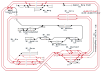
\includegraphics[width=\linewidth]{../images/plan.pdf}
  \caption{Schienennetz}
\end{figure}

\subsection{Tabelle}

\begin{table}[h]
\begin{center}
\begin{tabular}[h]{c|c|c}
ICE 1 & ICE 2 & ICE 3 \\ \hline
200 km/h & 250 km/h  & 300 km/h  \\
\end{tabular}
\caption{Sehr sehr schöne Tabelle}
\end{center}
\end{table} % implement chapter .tex file from the same folder
\newpage
\section{Berechnung des \Gls{fahrtverlauf}s} \label{kapitelFahrtverlauf}
Der \Gls{fahrtverlauf} eines Fahrzeuges wird bei der Berechnung in zwei verschiedenen Arten gespeichert. Einmal in so genannten \textit{\$keyPoints}, welche in einem Array die Start- und Zielgeschwindigkeit (\textit{time\_0} und \textit{time\_0}), die Start- und Endposition (\textit{position\_0} und \textit{position\_1}) und die Start- und Endzeit (\textit{time\_0} und \textit{time\_1}) einer Beschleunigung bzw. Verzögerung abspeichern. Für die Überprüfung, ob ein Fahrzeug die zulässige Höchstgeschwindigkeit in einem Infrastrukturabschnitt überschreitet, für die spätere Übermittlung der \Gls{echtzeitdaten} an das Fahrzeug und die exakte Positionsbestimmung, werden mittels der \textit{\$keyPoints} für jede Geschwindigkeitsänderungen (und bei konstanter Geschwindigkeit in 1 Meter Abständen) die aktuelle relative Position innerhalb eines Infrastrukturabschnitts, der Infrastrukturabschnitt, die aktuelle Zeit und die aktuelle Geschwindigkeit in einem Array gespeichert.
Der \Gls{fahrtverlauf} wird mit der Funktion \textit{updateNextSpeed$($$)$} berechnet, welche als Parameter unter anderem die Zugdaten aus dem \textit{\$allUsedTrains}-Array, Start- und Endzeit der Fahrt (\textit{\$startTime} und \textit{\$endTime}), den Ziel-Infrastrukturabschnitt (\textit{\$targetSection}) und die relative Position in dem Ziel-Infrastrukturabschnitt (\textit{\$targetPosition}) übergeben bekommt.
Die für die Berechnung benötigten Daten werden in den in Tabelle \ref{table:vars} beschriebenen Variablen gespeichert.
\begin{table}
\begin{center}
\renewcommand{\arraystretch}{1.2}
\begin{tabular}{c|c}
Bezeichnung & Funktion \\ \hline
\textit{\$keyPoint} (Array)                   			&   \makecell{Beschreibt eine Beschleunigung bzw.\\Verzögerung (\textit{position\_0}, \textit{position\_1},\\ \textit{time\_0}, \textit{time\_1}, \textit{speed\_0}, \textit{speed\_1})}           \\ \hline
\textit{\$next\_section} (Array)                  		&    IDs aller Abschnitte                  \\ \hline
\textit{\$next\_lenghts} (Array)                  		&    Längen aller Abschnitte                  \\ \hline
\textit{\$next\_v\_max} (Array)                  		&    Höchstgeschwindigkeit aller Abschnitte                  \\ \hline
\textit{\$indexCurrentSection} (Integer)             	&    Index des aktuellen Abschnitts               \\ \hline
\textit{\$indexTargetSection} (Integer)               	&    Index des Ziel-Abschnitts                  \\ \hline
\textit{\$cumulativeSectionLengthStart} (Array) 	&    Absolute Startposition aller Abschnitte                  \\ \hline
\textit{\$cumulativeSectionLengthEnd} (Array)  	&    Absolute Endposition aller Abschnitte                  \\ \hline
\textit{\$trainPositionChange} (Array)                	&    Alle absoluten Positionen des \Gls{fahrtverlauf}s                  \\ \hline
\textit{\$trainSpeedChange} (Array)                  	&   Alle Geschwindigkeiten des \Gls{fahrtverlauf}s                  \\
\end{tabular}
\renewcommand{\arraystretch}{1}
\caption{Beschreibung der verwendeten Variablen für die Fahrtverlaufsberechnung}
\label{table:vars}
\end{center}
\end{table}
In dem folgenden Abschnitt werden die einzelnen Schritte beschrieben, die durchlaufen werden um den optimalen \Gls{fahrtverlauf} zu berechnen. In der Darstellung \ref{fig:fahrtverlauf} wird der Ablauf grob schematisch dargestellt.
\begin{center}
\begin{figure}
\centering
\begin{tikzpicture}[node distance=1cm, auto,]
\node[punkt] (a) {Berechnung bei einer Beschleunigung auf die maximal mögliche Geschwindigkeit};
\node[below=of a, punkt] (b) {Wird die Geschwindigkeit in Infrastrukturabschnitten überschritten?};
\node[right=of b, punkt](c) {Neuberechnung unter Berücksichtigung der Geschwindigkeitsüberschreitung};
\node[below=of b, punkt] (d) {Wird die Mindestzeit auf einer Geschwindigkeit eingehalten?};
\node[right=of d, punkt](e) {Neuberechnung unter Berücksichtigung der Mindestzeit auf einer Geschwindigkeit};
\node[below=of d, punkt] (f) {Erreicht der Fahrzeug mit einer Verspätung das Ziel?};
\node[right=of f, punkt] (g) {Kann die Geschwindigkeit reduziert werden, ohne dass das Fahrzeug eine Verspätung hat?};
\node[below=of f, punkt] (h) {Übermittlung der \Gls{echtzeitdaten} an das Fahrzeug};
\node[right=of g, punkt] (i) {Reduzierung der Geschwindigkeit unter Einhaltung der Ankunfrtszeit};
\node[right=of a, punkt] (j) {Ist eine Fahrt ohne Gefahrenbremsung möglich?};
\node[right=of j, punkt] (k) {Berechnung der Gefahrenbremsung};
\node[above=of j, punkt] (l) {Start der Fahrtverlaufsberechnung};
\draw [pil] (a) -- (b);
\draw [pil] (b) --  node[pos=0.5] {Ja} (c);
\draw [pil] (c.north) -- +(0,0.5) -|  (b.north); 
\draw [pil] (b) -- node[pos=0.5,left] {Nein} (d);
\draw [pil] (d) --  node[pos=0.5] {Nein} (e);
\draw [pil] (e.north) -- +(0,0.3) -|  (d.north); 
\draw [pil] (d) -- node[pos=0.5,left] {Ja} (f);
\draw [pil] (f) -- node[pos=0.5] {Ja} (g);
\draw [pil] (f) -- node[pos=0.5,left] {Nein} (h);
\draw [pil] (g) -- node[pos=0.5] {Ja} (i);
\draw [pil] (g.south) -- node[pos=0.5,left] {Nein} +(0,-1) |-  (h.east); 
\draw [pil] (i.south) -- +(0,-1) |-  (h.east); 
\draw [pil] (j) -- node[pos=0.5,above] {Ja} (a);
\draw [pil] (j) -- node[pos=0.5] {Nein} (k);
\draw [pil] (l) -- (j);
\draw [pil] (k.east) -- +(0.5,0) |- (h.east);
\end{tikzpicture}
\caption{Ablaufplan der Fahrtverlaufsberechnung}
\label{fig:fahrtverlauf}
\end{figure}
\end{center}
\subsection{Ermittlung der Start- und Endposition der einzelnen Infrastrukturabschnitte unter Berücksichtigung der Zuglänge}
Für die Berechnung eines exemplarischen \Gls{fahrtverlauf}s wurden die in Tabelle \ref{table:infraex} definierten Infrastrukturabschnitte benutzt. Diese Abschnitte wurden so gewählt, sodass alle Funktionen und die Allgemeingültigkeit des Algorithmus gezeigt werden können und treten so im \ac{ebuef} nicht auf. 
\begin{table}
\begin{center}
\renewcommand{\arraystretch}{1.2}
\begin{tabular}{c| C{3cm} |c}
Infrastrukturabschnitts-ID & Länge & zulässige Höchstgeschwindigkeit \\ \hline
1000                   &   300 $m$    & 120 $km/h$                        \\ \hline
1001                  &    400 $m$   & 120 $km/h$                        \\ \hline
1002                   &   300 $m$    &        120 $km/h$                         \\ \hline
1003                   &    400 $m$   &         90 $km/h$                        \\ \hline
1004                   &    300 $m$   &            60 $km/h$                     \\ \hline
1005                   &   200 $m$    &           60 $km/h$                      \\ \hline
1006                   &  400 $m$     &      90 $km/h$                           \\ \hline
1007                   &  500 $m$     &      120 $km/h$                           \\ \hline
1008                   &   300 $m$    &      120 $km/h$                           \\ \hline
1009                   &   400 $m$    &      100 $km/h$                           \\ \hline
1010                   &   300 $m$    &      60 $km/h$                           \\ \hline
1011                   &   300 $m$    &         40 $km/h$                        \\ 
\end{tabular}
\renewcommand{\arraystretch}{1}
\caption{Exemplarische Infrastrukturabschnitte}
\label{table:infraex}
\end{center}
\end{table}
Als exemplarisch gewählte Zugdaten wurden die in Tabelle \ref{table:train-ex} definierten Daten verwendet.
\begin{table}[]
\begin{center}
\renewcommand{\arraystretch}{1.2}
\begin{tabular}{r L{3cm}}
relative Startposition                   &   10 $m$                         \\ 
relative Zielposition                  &    290 $m$                         \\ 
aktueller Infrastrukturabschnitt                   &   1001                         \\ 
Ziel-Infrastrukturabschnitt                  &    1010                         \\ 
Startgeschwindigkeit                   &   0 $km/h$                          \\ 
Zielgeschwindigkeit                   &    0 $km/h$                        \\ 
Zuglänge                   &    50 $m$                        \\ 
Bremsverzögerung                   &    0,8 $m/s^{2}$                        \\ 
Fahrplan vorhanden                   &    ja                        \\ 
Zeit bis zur nächsten Betriebsstelle                   &    210 $s$                        \\ 
\end{tabular}
\renewcommand{\arraystretch}{1}
\caption{Exemplarische Zugdaten}
\label{table:train-ex}
\end{center}
\end{table}
Die zuvor ermittelten nächsten Infrastrukturabschnitte inklusive derer Längen und zulässigen Höchstgeschwindigkeit müssen für die Berechnung des \Gls{fahrtverlauf}s angepasst werden, da ein Fahrzeug erst beschleunigen darf, wenn das komplette Fahrzeug in den Infrastrukturabschnitt eingefahren ist. In Darstellung \ref{fig:it1} sind die Infrastrukturabschnitte dargestellt, so wie sie von dem Fahrzeug ermittelt wurden. Dabei werden alle Abschnitte, die das Fahrzeug schon durchfahren hat oder hinter dem Zielabschnitt liegen nicht dargestellt. Zudem wird in dem aktuellen Abshcnitt die relative Position von der Länge abgezogen und in der Zielabschnitt wird nur bis zur relativen Zielposition abgebildet. Dementsprechend ist der erste Abschnitt in der Darstellung \ref{fig:it1} der Abschnitt mit der ID 1001. Dieser hat aufgrund der aktuellen relativen Position des Fahrzeugs eine Länge von 290 $m$. Und der letzte Abschnitt ist der Abschnitt mit der ID 1010 und einer Länge von ebenfalls 290 $m$.
\begin{figure}
  \includegraphics[width=\linewidth]{../images/matlab/it1.pdf}
  \caption{Darstellung der Infrastrukturabschnitte und die zugehörige Höchstgeschwindigkeit}
  \label{fig:it1}
\end{figure}
Bei der Berücksichtigung der Fahrzeuglänge wird durch alle Infrastrukturabschnitt iteriert und die Zuglänge auf die Länge das Abschnitts addiert. Von dieser neu ermittelten Endposition des Abschnitts wird überprüft, ob zwischen der vorherigen Endposition und der neu ermittelten Endposition ein Infrastrukturabschnitt liegt, dessen zulässige Höchstgeschwindigkeit geringer ist, als die des ursprünglichen Abschnitts. Wenn dieser Fall eintritt, wird der Abschnitt nur so weit verlängert, sodass keine Höchstgeschwindigkeit der folgenden Abschnitte überschritten wird. Von der neu ermittelten Endposition wird überprüft, in welchem Abschnitt diese liegt und mit dem Abschnitt wird dann weiter gerechnet. Sobald der Ziel-Abschnitt erreicht wurde, wird die Schleife abgebrochen. Die neu ermittelten Abschnitte werden in den Arrays \textit{\$next\_lengths\_mod} und \textit{\$next\_v\_max\_mod} abgespeichert. Durch diese Algorithmus kann es dazu kommen, dass sich die Anzahl der Abschnitte verändert hat. Dementsprechend können die Abschnitte nicht mehr eindeutig mit der Infrastruktur-ID bezeichnet werden. Mittels \textit{\$next\_lengths\_mod} und \textit{\$next\_v\_max\_mod} werden mit der Funktion \textit{createCumulativeSections$($$)$} für jeden Abschnitt die absolute Start- und Endposition in den Arrays \textit{\$cumulativeSectionLengthStartMod} und \textit{\$cumulativeSectionLengthEndMod} gespeichert. Diese Umwandlung ist essentiell für die Überprüfung, in welchem Abschnitt ein Fahrzeug sich aktuell befindet. Die neu berechneten Abschnitte werden sind in der Darstellung \ref{fig:it2} in rot abgebildet und beschreiben die maximale Geschwindigkeit, die ein Fahrzeug fahren darf an der jeweiligen Position.
\begin{figure}
\includegraphics[width=\linewidth]{../images/matlab/it2.pdf}
\caption{Darstellung Infrastrukturabschnitte und die zugehörige Höchstgeschwindigkeit unter Berücksichtigung der Fahrzeuglänge}
\label{fig:it2}
\end{figure}
\subsection{Berechnung bei einer Beschleunigung auf die maximal mögliche Geschwindigkeit} \label{v_max}
Im ersten Schritt für die Distanz zwischen der aktuellen Position und der Ziel-Position mittels \textit{\$cumulativeSectionLengthStart}, \textit{\$cumulativeSectionLengthEnd}, \textit{\$indexCurrentSection} und \textit{\$indexTargetSection} berechnet. Für diese Distanz und die Startgeschwindigkeit wird mit Hilfe der Funktion \textit{getVMaxBetweenTwoPoints$($$)$} (Code-Beispiel ~\ref{lst:getVMaxBetweenTwoPoints}) die maximale Geschwindigkeit ermittelt, die das Fahrzeug aufnehmen kann, um noch bis zum Ziel rechtzeitig bremsen zu können. Dabei wird in 10 $km/h$-Schritten iteriert und der maximale Wert zurückgegeben. Innerhalb der Funktion wir die Funktion \textit{getBrakeDistance$($$)$} (Code-Beispiel ~\ref{lst:getBrakeDistance}) aufgerufen, welche die benötigte Distanz für eine Beschleunigung bzw. Verzögerung berechnet. 
\begin{figure}
\begin{lstlisting}[caption={\textit{getVMaxBetweenTwoPoints$($$)$}},captionpos=b,label={lst:getVMaxBetweenTwoPoints}]
function getVMaxBetweenTwoPoints(float $distance, int $v_0, int $v_1) {
	global $verzoegerung;
	global $globalFloatingPointNumbersRoundingError;
	$v_max = array();
	for ($i = 0; $i <= 120; $i = $i + 10) {
		if ((getBrakeDistance($v_0, $i, $verzoegerung) + getBrakeDistance($i, $v_1, $verzoegerung)) < ($distance + $globalFloatingPointNumbersRoundingError)) {
			array_push($v_max, $i);
		}
	}
	if (sizeof($v_max) == 0) {
		if ($v_0 == 0 && $v_1 == 0 && $distance > 0) {
			echo "Der zug müsste langsamer als 10 km/h fahren, um das Ziel zu erreichen.";
		} else {
			// TODO: Notbremsung
		}
	} else {
		if ($v_0 == $v_1 && max($v_max) < $v_0) {
			$v_max = array($v_0);
		}
	}
	return max($v_max);
}
\end{lstlisting}
\end{figure}
\begin{figure}
\begin{lstlisting}[caption={\textit{getBrakeDistance$($$)$}},captionpos=b,label={lst:getBrakeDistance}]
function getBrakeDistance (float $v_0, float $v_1, float $verzoegerung) {
	if ($v_0 > $v_1) {
		return $bremsweg = 0.5 * ((pow($v_0/3.6,2)-pow($v_1/3.6, 2))/($verzoegerung));
	} if ($v_0 < $v_1) {
		return $bremsweg = -0.5 * ((pow($v_0/3.6,2)-pow($v_1/3.6, 2))/($verzoegerung));
	} else {
		return 0;
	}
}
\end{lstlisting}
\end{figure}
Durch die gegebene Startgeschwindigkeit und die höchstmögliche Geschwindigkeit wird ein erster \Gls{fahrtverlauf} berechnet. Dabei werden zwei \textit{\$keyPoints} erzeugt. Mithilfe der Funktion \textit{createTrainChanges$($$)$} wird aus diesen beiden \textit{\$keyPoints} für jede Geschwindigkeitsveränderung die aktuelle absolute Position und Geschwindigkeit ermittelt. An den Positionen, an den das Fahrzeug eine konstante Geschwindigkeit hat, wird in 1 Meter Abständen die absolute Position und die Geschwindigkeit gespeichert. Die ermittelten Daten werden in den Arrays \textit{\$trainPositionChange} und \textit{\$trainSpeedChange} gespeichert. In der Darstellung \ref{fig:it3} ist das Ergebnis der 1. Iteration abgebildet.
\begin{figure}
\includegraphics[width=\linewidth]{../images/matlab/it3.pdf}
\caption{Fahrtverlaufberechnung (1. Iteration)}
\label{fig:it3}
\end{figure}
\subsection{Überprüfung des \Gls{fahrtverlauf}s nach Geschwindigkeitsüberschreitungen} \label{überprüfung}
Für die Überprüfung, ob bei einem \Gls{fahrtverlauf} in manchen Infrastrukturabschnitten die zulässige Höchstgeschwindigkeit überschritten wird, wird nach jeder Berechnung die Funktion \textit{checkIfTrainIsToFastInCertainSections$($$)$} (Code-Beispiel ~\ref{lst:checkIfTrainIsToFastInCertainSections}) aufgerufen. In dieser Funktion wird über alle absoluten Positionen (\textit{\$trainPositionChange}) iteriert, überprüft in welchem Abschnitt sich diese Position befindet und überprüft, ob die zugehörige Geschwindigkeit aus dem \textit{\$trainSpeedChange}-Array die zulässige Höchstgeschwindigkeit überschreitet. Sobald in einem Abschnitt eine Geschwindigkeitsüberschreitung vorliegt, wird der zugehörige Index des Abschnitts in dem \textit{\$faildSections}-Array gespeichert. Diese Abschnitte sind in der Darstellung \ref{fig:it3} Lila hinterlegt. Als Rückgabewert der Funktion wird wird ein Array wiedergegeben, welches abspeichert, ob es zu einer Geschwindigkeitsüberschreitung gekommen ist (\textit{\grqq{}failed\grqq{}}) und wenn das der Fall ist auch die Indexe der Abschnitte (\textit{\grqq{}failed\_sections\grqq{}}).
\begin{figure}
\begin{lstlisting}[caption={\textit{checkIfTrainIsToFastInCertainSections$($$)$}},captionpos=b,label={lst:checkIfTrainIsToFastInCertainSections}]
function checkIfTrainIsToFastInCertainSections() {
	global $trainPositionChange;
	global $trainSpeedChange;
	global $cumulativeSectionLengthStartMod;
	global $next_v_max_mod;
	global $indexTargetSectionMod;
	$faildSections = array();
	foreach ($trainPositionChange as $trainPositionChangeKey => $trainPositionChangeValue) {
		foreach ($cumulativeSectionLengthStartMod as $cumulativeSectionLengthStartKey => $cumulativeSectionLengthStartValue) {
			if ($trainPositionChangeValue < $cumulativeSectionLengthStartValue) {
				if ($trainSpeedChange[$trainPositionChangeKey] > $next_v_max_mod[$cumulativeSectionLengthStartKey - 1]) {
					array_push($faildSections, ($cumulativeSectionLengthStartKey -1));
				}
				break;
			} else if ($cumulativeSectionLengthStartKey == $indexTargetSectionMod) {
				if ($trainPositionChangeValue > $cumulativeSectionLengthStartValue) {
					if ($trainSpeedChange[$trainPositionChangeKey] > $next_v_max_mod[$cumulativeSectionLengthStartKey]) {
						array_push($faildSections, $cumulativeSectionLengthStartKey);
					}
					break;
				}
			}
		}
	}
	if (sizeof($faildSections) == 0) {
		return array("failed" => false);
	} else {
		return array("failed" => true, "failed_sections" => array_unique($faildSections));
	}
}
\end{lstlisting}
\end{figure}
\subsection{Neuberechnung unter Berücksichtigung der Geschwindigkeitsüber-\\schreitung}  \label{neuberechnung}
In dem Fall, dass es zu einer Geschwindigkeitsüberschreitung gekommen ist, wird der \Gls{fahrtverlauf} neu berechnet. Als Grundlage dafür diesen die \textit{\grqq{}failed\_sections\grqq{}} aus der \textit{check\-If\-Train\\Is\-To\-Fast\-In\-Certain\-Sections$($$)$} Funktion (Code-Beispiel ~\ref{lst:checkIfTrainIsToFastInCertainSections}). Die Funktion \textit{recalculate\-Key\-Points$($$)$} vergleicht immer zwei benachbarte \textit{\$keyPoints} und berechnet in dem Fall einer Geschwindigkeitsüberschreitung mit der Funktion \textit{checkBetweenTwoKeyPoints$($$)$} diese neu. In dem Fall, dass zwischen zwei benachbarten \textit{\$keyPoints} die zulässige Höchstgeschwindigkeit überschritten wird, wird die absolute Start- und End-Position dieser Geschwindigkeitsüberschreitung gespeichert. Im folgenden Schritt wird wie in dem Abschnitt \ref{v_max} zwischen den Start-Werten des ersten \textit{\$keyPoints} und der ersten Geschwindigkeitsüberschreitung die maximale Geschwindigkeit berechnet und zwei neue \textit{\$keyPoints} erzeugt. Das gleiche passiert zwischen der Position der letzten Geschwindigkeitsüberschreitung und den End-Werten des zweiten \textit{\$keyPoints}. Dadurch wird sichergestellt, dass es immer eine gerade anzahl an \textit{\$keyPoints} gibt und somit in jedem Iterationsschritt zwei benachbarte \textit{\$keyPoints} verglichen werden können. Nachdem alle \textit{\$keyPoint}-Paare überprüft werden, werden mit Hilfe der \textit{createTrainChanges$($$)$} Funktion die Arrays \textit{\$trainPositionChange} und \textit{\$trainSpeedChange} erzeugt. Dieser neu berechnete \Gls{fahrtverlauf} wird dann wieder der Funktion \textit{checkIfTrain\\IsToFastInCertainSections$($$)$} Funktion (Code-Beispiel ~\ref{lst:checkIfTrainIsToFastInCertainSections}) übergeben. Dieser Prozess wird solange durchlaufen, bis es zu keiner Geschwindigkeitsüberschreitung mehr kommt. In den folgenden Abbildungen (Darstellung \ref{fig:it4}, \ref{fig:it5} und \ref{fig:it6}) werden die Ergebnisse der einzelnen Iterationsschritte visuell abgebildet, wobei die grau gepunkteten Linien die Ergebnisse der vorherigen Iterationsschritte darstellen.
\begin{figure}
\includegraphics[width=\linewidth]{../images/matlab/it4.pdf}
\caption{Fahrtverlaufberechnung (2. Iteration)}
\label{fig:it4}
\end{figure}
\begin{figure}
\includegraphics[width=\linewidth]{../images/matlab/it5.pdf}
\caption{Fahrtverlaufberechnung (3. Iteration)}
\label{fig:it5}
\end{figure}
\begin{figure}
\includegraphics[width=\linewidth]{../images/matlab/it6.pdf}
\caption{Fahrtverlaufberechnung (4. Iteration)}
\label{fig:it6}
\end{figure}
\subsection{Einhaltung der Mindestzeit auf einer Geschwindigkeit} \label{minTime}
\begin{enumerate}
\item Ideal: möglichst späte v reduzieren
\end{enumerate}
Für eine möglichst realitätsnahe Simulation kann über die Variable \textit{\$globalTimeOnOneSpeed} in der Datei \textit{globalVariables.php} eine Mindestzeit festgelegt werden, die ein Fahrzeug auf einer Geschwindigkeit mindestens einhalten muss. Ebenfalls kann über die Variablen \textit{\$useMinTimeOnSpeed} und \textit{\$errorMinTimeOnSpeed} festgelegt werden, ob die Funktion aktiviert sein soll und ob es in dem Fall, dass diese Zeit nicht eingehalten werden kann, zu einer Fehlermeldung kommen soll. Im Falle einer Fehlermeldung würde das Fahrzeug nicht losfahren bzw. eine Gefahrenbremsung einleiten, falls das Fahrzeug aktuell eine Geschwindigkeit $v > 0$ hat. 
Wenn auf einem Abschnitt die Mindestzeit nicht eingehalten werden kann, kann eine Beschleunigung später eingeleitet werden, eine Verzögerung vorzeitiger eingeleitet werden oder auf eine kleinere Geschwindigkeit beschleunigt werden. In dem folgenden Algorithmus werden die \dots
Dadurch, dass sich eine Verschiebung einer Beschleunigung bzw. Verzögerung auf die nächsten Abschnitte auswirken kann, wird der \Gls{fahrtverlauf} in \textit{\$subsections} unterteilt. Eine \textit{\$subsection} beschreibt dabei den Bereich des \Gls{fahrtverlauf}s, in dem das Fahrzeug zum ersten Mal beschleunigt und zum letzten Mal abbremst. In der Darstellung \ref{fig:it7} wurde der exemplarische \Gls{fahrtverlauf} somit in zwei \textit{\$subsection} unterteilt, welche Lila bzw. Gelb hinterlegt sind.
\begin{figure}
\includegraphics[width=\linewidth]{../images/matlab/it7.pdf}
\caption{Einteilung des \Gls{fahrtverlauf}s in \textit{\$subsections}}
\label{fig:it7}
\end{figure}
Diese Einteilung wird vorgenommen, da sich die Verschiebung einer Beschleunigung bzw. Verzögerung auf die folgenden bzw. vorherigen Abschnitte auswirkt. Durch diese Einteilung kann verhindert werden, dass es dadurch zu Konflikten kommt. Falls die Beschleunigungen bzw. Verzögerungen soweit nach hinten bzw. nach vorne verschoben werden müssen, kann die maximale Geschwindigkeit auf dieser \textit{\$subsection} reduziert werden und die zur Verfügung stehende Strecke vergrößert werden. Wie in Darstellung \ref{fig:it7} zu erkennen wird hierbei im ersten Schritt der Abschnitt zwischen zwei \textit{\$subsections} ausgelassen. Nach der Ermittlung der \textit{subsections} wird überprüft, ob auf den Abschnitten zwischen den \textit{\$subsections} die Mindestzeit eingehalten wird. Wenn das nicht der Fall ist, wird der Abschnitt automatisch dem in Fahrtrichtung hinteren \textit{\$subsection} zugeordnet. Dadurch wird sichergestellt, dass das Fahrzeug, wenn es an einer Stelle des \Gls{fahrtverlauf}s die Geschwindigkeit reduziert, dies möglichst spät tut.
Nachdem die \textit{\$subsections} mittels der Funktion \textit{createSubsections$($$)$} erstellt wurden und mit der Funktion \textit{array\_reverse$($$)$} in umgekerte Reihenfolge in dem Array \textit{\$subsection\_list} gesammelt wurden, wird für jede \textit{\$subsection} überprüft, ob die Beschleunigungen bzw. Verzögerungen verschoben werden können. Dabei wird über alle konstanten Geschwindigkeiten iteriert, überprüft, ob die Mindestzeit eingehalten wird und wenn das nicht der Fall ist, wird überprüft, ob eine Verschiebung möglich ist. Sollte bei einer Verschiebung die $position\_1$ des \textit{\$keyPoints} hinter $position\_0$ des zweiten \textit{\$keyPoints} liegen (bei einer Beschleunigung), wird der zweite \textit{\$keyPoint} gelöscht. Gleiches geschieht bei der Verzögerung in umgekehrter Reihenfolge. Nach der Verschiebung wird überprüft, ob auf allen konstanten Geschwindigkeit die Mindestzeit eingehalten wird. Wenn das der Fall ist, wird die nächste \textit{\$subsection} überprüft. In dem Fall, dass durch die Verschiebung die Mindestzeit nicht eingehalten werden kann, wird die maximale Geschwindigkeit auf dieser \textit{\$subsection} um $10 km/h$ reduziert, die \textit{\$subsections} neu berechnet und erneut über alle \textit{\$subsection} iteriert. Die Neuberechnung ist notwendig, da durch die Reduzierung der Geschwindigkeit die \textit{\$subsections} anders aufgeteilt sein können.
Wenn alle \textit{\$subsections} die Mindestzeit einhalten, wird der Algorithmus beendet. In der Darstellung \ref{fig:it9} ist der \Gls{fahrtverlauf} unter Einhaltung der Mindestzeit auf einer Geschwindigkeit abgebildet.
\begin{figure}
\includegraphics[width=\linewidth]{../images/matlab/it9.pdf}
\caption{Fahrtverlauf unter Einhaltung der Mindestzeit}
\label{fig:it9}
\end{figure}
\begin{table}
\begin{center}
\renewcommand{\arraystretch}{1.2}
\begin{tabular}{c|c}
Index & Funktion \\ \hline
\textit{max\_index}                 	&  	\makecell{ndex des \textit{\$keyPoints} mit der Beschleunigung auf die\\maximale Geschwindigkeit in der \textit{\$subsection}}     \\ \hline
\textit{indexes}                 		&    	Indexe aller beinhalteten \textit{\$keyPoints}                  \\ \hline
\textit{is\_prev\_section}           	&   	Berücksichtigung des Abschnitts vor der \textit{\$subsection}     \\ \hline
\textit{is\_next\_section}           	&     	Berücksichtigung des Abschnitts nach der \textit{\$subsection}                 \\ \hline
\textit{failed}                 		&   	Unterschreitung der Mindestzeit auf der \textit{\$subsection}     \\ 
\end{tabular}
\renewcommand{\arraystretch}{1}
\caption{Aufbau des \textit{\$subsection}-Arrays}
\label{table:subsection}
\end{center}
\end{table}
Für den Fall, dass das Fahrzeug auf einer Geschwindigkeit die Mindestzeit nicht einhält und als nächstes beschleunigen würde, kann die Beschleunigung später eingeleitet werden. 
\subsection{Berücksichtigung der Ankunftszeit bei der Berechnung des \Gls{fahrtverlauf}s} \label{time}
Der berechnete \Gls{fahrtverlauf} in den Kapiteln \ref{v_max}, \ref{überprüfung}, \ref{neuberechnung} und \ref{minTime} ermittelt die frühstmögliche Ankunftszeit am Ziel. In dem Fall, dass der Zug dadurch mit einer Verspätung am Ziel ankommt wird der \Gls{fahrtverlauf} an das Fahrzeug übergeben. Falls der Zug allerdings mit dem \Gls{fahrtverlauf} zu früh am Ziel ankommen würde, wird überprüft, ob es möglich ist die Geschwindigkeit zu reduzieren, sodass der Zug energieeffizienter fahren kann und ohne Verspätung am Ziel ankommt.
Ergebnis ist in \ref{fig:it9} abgebildet.
Im ersten Schritt wird mittels der Funktion \textit{checkIfTheSpeedCanBeDecreased$($$)$} überprüft, ob die Geschwindigkeit reduziert werden kann. Dabei werden alle \textit{\$keyPoints} ermittelt, bei denen das Fahrzeug beschleunigt und die beim darauffolgenden \textit{\$keyPoint} abbremsen. Für jeden dieser \textit{\$keyPoints} werden die möglichen Geschwindigkeiten ermittelt, welche das Fahrzeug zwischen den beiden \textit{\$keyPoints} fahren könnte. Für die Berechnung dieser Geschwindigkeiten wird als niedrigste Geschwindigkeit die \textit{speed\_0} des ersten \textit{\$keyPoints} bzw. \textit{speed\_1} des zweiten \textit{\$keyPoints} - jenachdem, welche niedriger ist - genommen und in 10 $km/h$-Schritten bis  \textit{speed\_1} des ersten \textit{\$keyPoints} abgespeichert. Daraus ergibt sich für jeden \textit|{\$keyPoint} eine \textit{range} an möglichen Geschwindigkeiten. Als Rückgabewert der Funktion wird ein \textit{Array} wiedergegeben, welches die Einträge \textit{possible} und \textit{range} enthält und als \textit{\$returnSpeedDecrease} abgespeichert. Der Eintrag \textit{possible} gibt an, ob das Fahrzeug auf dem gesamten \Gls{fahrtverlauf} die Geschwindigkeit reduzieren könnte und wird als Boolescher Wert (\textit{true}/\textit{false}) abgespeichert und und in dem \textit{Array} \textit{range} werden alle Indexe der möglichen \textit{\$keyPoints} inklusive der ermittelten Geschwindigkeiten abgespeichert.
In dem in Abbildung \ref{fig:it9} dargestellten \Gls{fahrtverlauf} wären so für den \textit{\$keyPoint} mit dem Index 0 (die Indexe der \textit{\$keyPoints} entsprechen dem Zahlenbereich der $\mathbb{N}_0$) die Geschwindigkeiten 60, 70 und 80 $km/h$ ermittelt worden und für den \textit{\$keyPoint} mit dem Index $2$ die Geschwindigkeiten 60, 70, 80 und 90 $km/h$.
Wenn eine Reduzierung der Geschwindigkeit möglich ist, wird in einer \textit{while}-Schleife versucht die Geschwindigkeit zu reduzieren, bis das Fahrzeug bei der nächsten Reduzierung mit einer Verspätung am Ziel ankommen würde oder eine weitere Reduzierung nicht möglich ist, da die Maximalgeschwindigkeit auf dem \Gls{fahrtverlauf} 10 $km/h$ beträgt. Innerhalb der \textit{while}-Schleife ermittelt die Funktion \textit{findMaxSpeed$($$)$} aus dem \textit{\$returnSpeedDecrease}-Array den \textit{\$keyPoint} mit der höchsten Geschwindigkeit. Für den Fall, dass mehrere \textit{\$keyPoints} die selbe Höchstgeschwindigkeit haben, wird der letzte dieser \textit{\$keyPoints} ermittelt. Im Anschluss wird mit einer \textit{for}-Schleife in 10er-Schritten in absteigender Reihenfolge über die möglichen Geschwindigkeiten iteriert und überprüft, ob durch die Anpassung die Ankunftszeit eingehalten werden kann. Sobald die Ankunftszeit nicht eingehalten werden kann, werden die \textit{\$keyPoints} aus dem vorherigen Iterationsschritt gespeichert und die \textit{while}-Schleife wird abgebrochen. Sollte die \textit{for}-Schleife durchlaufen, ohne dass es zu einer Überschreitung der maximal verfügbaren Zeit kommt, wird die Funktion \textit{checkIfTheSpeedCanBeDecreased$($$)$} erneut aufgerufen. 
Das Ergebnis dieser Berechnung ist in der Abbildung \ref{fig:it10} zu sehen.
\begin{figure}
\includegraphics[width=\linewidth]{../images/matlab/it10.pdf}
\caption{\Gls{fahrtverlauf} mit reduzierter Geschwindigkeit unter Einhaltung der Ankunftszeit}
\label{fig:it10}
\end{figure}
\subsection{Berücksichtigung der exakten Ankunftszeit bei der Berechnung des \Gls{fahrtverlauf}s} \label{time2}
Die in Kapitel \ref{minTime} errechnete Ankunftszeit, beschreibt die spätmöglichste Ankunftszeit am Ziel, ohne dass das Fahrzeug mit einer Verspätung am Ziel ankommt, wenn bei einer Beschleunigung auf eine geringere Zielgeschwindigkeit beschleunigt wird. Dadurch wird das Fahrzeug im Normalfall noch nicht exakt pünktlich das Ziel erreichen. Über die Variable \textit{\$useSpeedFineTuning} kann festgelegt werden, ob das Fahrzeug eine exakte Ankunftszeit versuchen soll zu erreichen. Wenn diese Funktion aktiviert ist und der Eintrag \textit{possible} aus dem Array \textit{\$returnSpeedDecrease} \textit{true} ist, wird für den letzten \textit{\$keyPoint} aus dem \textit{\$returnSpeedDecrease}-Array überprüft, ob die Verzögerung des nächsten \textit{\$keyPoints} vorzeitiger eingeleitet werden kann. Sollte die Zielgeschwindigkeit der Verzögerung 0 $km/h$ sein, wird die Verzögerung unterteilt in eine Verzögerung auf 10 $km/h$ und eine von 10 $km/h$ auf 0 $km/h$. Die Position der vorzeitig eingeleiteten Verzögerung wird mittels der Funktion \textit{speedFineTuning$($$)$} berechnet, welche als Parameter den Betrag der Differenz zwischen aktueller Soll- und Ist-Ankunftszeit und den Index des vorherigen \textit{\$keyPoints} übergeben bekommt.
\begin{figure}
\includegraphics[width=\linewidth]{../images/matlab/it11.pdf}
\caption{speedFineTuning\_1}
\label{fig:it11}
\end{figure}
In Abbildung \ref{fig:it11} werden die Geschwindigkeiten ($v_1$,$v_2$), Strecken ($s_1$,$s_2$) und Zeiten ($t_1$,$t_2$) vor und nach der Verzögerung, welche vorzeitiger eingeleitet werden soll, um eine pünktliche Ankunft am Ziel zu ermöglichen, dargestellt und in Tabelle \ref{table:speed_fine_tuning_ex} sind die exakten Werte des exemplarischen \Gls{fahrtverlauf}s aufgelistet, damit die verwendete Gleichung (Gleichung \ref{eq:t_1_tuning} aus Kapitel \ref{formula}) an diesem Beispiel angewandt werden kann. In diesem konkreten Beispiel würde das Fahrzeug 3,31 $s$ ($t_{\varDelta}$) zu früh an der Haltestelle ankommen, wodurch das Fahrzeug für die Zurücklegung der Strecken $s_1$ und $s_2$ insgesamt 85,42$s$ ($t_{ges}=t_1+t_2+t_{\varDelta}$) zur Verfügung hat.
\begin{table}
\begin{center}
\renewcommand{\arraystretch}{1.2}
\begin{tabular}{r L{3cm}}
$v_1$                   &   70 $km/h$ (19,44$m/s$)                         \\ 
$v_2$                   &   60 $km/h$ (16,67$m/s$)                         \\ 
$s_1$                   &   1207,67 $m$                         \\ 
$s_2$                   &   333,33 $m$                         \\ 
$s_{ges}$                   &   1541 $m$                         \\ 
$t_1$                   &   62,11 $s$                         \\ 
$t_2$                   &   20 $s$                         \\ 
$t_{\varDelta}$                   &   3,31 $s$                         \\ 
$t_{ges}$                   &   85,42 $s$                         \\ 
\end{tabular}
\renewcommand{\arraystretch}{1}
\caption{Geschwindigkeiten, Strecken und Zeiten vor und nach der Verzögerung}
\label{table:speed_fine_tuning_ex}
\end{center}
\end{table}
Durch das Einsetzen dieser Werte in die Gleichung \ref{eq:t_1_tuning} aus dem Kapitel \ref{formula} ergibt sich für $t_3$ ($t_3$, $t_4$, $s_3$ und $s_4$ bezeichnen die Strecken und Zeiten nach der Anpassung) ein Wert von 42,2$s$. Dementsprechend muss die Verzögerung 19,85$s$ ($t_1$ - $t_3$) früher eingeleitet werden
\begin{figure}
\[t_{3} = \frac{1541m - 16,67 m/s \cdot 85,42 s}{19,44 m/s - 16,67 m/s}\]
%\[t_{3} = \frac{1541m - 1423,95 m}{2,77 m/s}\]
%\[t_{3} = \frac{117,05 m}{2,77 m/s}\]
\[t_{3} = 42,26 s\]
\end{figure}
Die vorzeitige Einleitung der Verzögerung sorgt dafür, dass das Fahrzeug seinen nächsten Haltepunkt genau pünktlich erreicht und ist in Abbildung \ref{fig:it12} dargestellt, wobei durch die gepunktete Linie der \Gls{fahrtverlauf} vor der Anpassung zu sehen ist. Die neu berechneten Werte sind in Tabelle \ref{table:speed_fine_tuning_ex_2} aufgelistet.
\begin{figure}
  \includegraphics[width=\linewidth]{../images/matlab/it12.pdf}
  \caption{speedFineTuning\_2}
  \label{fig:it12}
\end{figure}
\begin{table}
\begin{center}
\renewcommand{\arraystretch}{1.2}
\begin{tabular}{r L{3cm}}
$s_3$                   	&   821,91$m$                      	\\ 
$s_4$                   	&   719,1$m$                         	\\ 
$t_3$                   	&   42,26$s$                         	\\ 
$t_4$                   	&   43,16$s$                         	\\ 
%$t_{ges}$           	&   85,42 $s$                         	\\ 
\end{tabular}
\renewcommand{\arraystretch}{1}
\caption{Geschwindigkeiten, Strecken und Zeiten vor und nach der Verzögerung nach der Anpassung}
\label{table:speed_fine_tuning_ex_2}
\end{center}
\end{table}
Der finale \Gls{fahrtverlauf} ist in Abbildung \ref{fig:it13} dargestellt und kann so dem Fahrzeug übergeben werden.
\begin{figure}
  \includegraphics[width=\linewidth]{../images/matlab/it13.pdf}
  \caption{Finaler \Gls{fahrtverlauf}}
  \label{fig:it13}
\end{figure}
\subsection{Einleitung einer Gefahrenbremsung} \label{notbremsung}
Eine Gefahrenbremsung wird eingeleitet, sobald ein Fahrzeug bei einer sofortigen Verzögerung ein auf Halt stehendes Signal überfahren würde, in einem Infrastruktur-Abschnitt die zulässige Höchstgeschwindigkeit überschreiten würde oder an dem nächsten planmäßigen Halt nicht rechtzeitig zum stehen kommen würde. Bei einer Gefahrenbremsung wird mit einer Notbremsverzögerung von 2$m/s^2$ abgebremst. Dieser Wert kann in der Datei \textit{globalVariables.php} über die Variable \textit{\$globalNotverzoegerung} angepasst werden. Für eine möglichst realitätsnahe Simulation einer Gefahrenbremsung, bei der das Risiko für Fahrzeugschäden möglichst gering ist, wurde sich dafür entschieden, dass die Fahrzeuge, wenn sie an der Gefahrenstelle eine Geschwindigkeit haben, für die gilt: $v\geq10km/h$, nach der Geschwindigkeit von 10$km/h$ direkt die Geschwindigkeit von 0$km/h$ übermittelt bekommen. Dadurch wird bei der Berechnung einer Gefahrenbremsung zwischen drei Fällen unterschieden:
\begin{enumerate}
\item Fahrzeug hält mit der Notbremsverzögerung vor der Gefahrenstelle
\item Fahrzeug hat bei der Gefahrenstelle eine Geschwindigkeit von $v<10km/h$
\item Fahrzeug hat bei der Gefahrenstelle eine Geschwindigkeit von $v\geq10km/h$
\end{enumerate}
Für die Überprüfung, ob das Fahrzeug mit der Notbremsverzögerung vor der Gefahrenstelle zum Stehen kommt, wird mittels der Funktion \textit{getBrakeDistance$($$)$} der Bremsweg ($s_{Bremsweg}$) berechnet und mit der Distanz zur Gefahrenstelle ($s_{Gefahrenstelle}$) verglichen. Sollte für den Bremsweg gelten: $s_{Bremsweg}\leq s_{Gefahrenstelle}$, wird das Fahrzeug die Gefahrenbremsung einleiten und in 2$km/h$-Schritten auf 0$km/h$ abbremsen. In dem Fall, dass der Bremsweg länger als die Strecke bis zur Gefahrenstelle ist, wird überprüft, welche Geschwindigkeit das Fahrzeug an der Gefahrenstelle hat. Für diese Berechnung wird die Gleichung \ref{eq:gefahrenbremsung} aus dem Kapitel \ref{formula} verwendet. Sollte das Fahrzeug an der Gefahrenstelle eine Geschwindigkeit von $v\geq10km/h$ haben, bremst das Fahrzeug in 2$km/h$-Schritten auf 10$km/h$ ab und bekommt nach der Übermittlung der 10$km/h$ direkt 0$km/h$ übergeben. In dem Fall, dass das Fahrzeug an der Gefahrenstelle langsamer als 10$km/h$ ist, bremst das Fahrzeug wie im 1. Fall in 2$km/h$-Schritten auf 0$km/h$ ab. Bei einer Gefahrenbremsung bekommt das jeweilige Fahrzeug eine Fehlermeldung übermittelt und wird nicht weiterfahren. Das liegt daran, dass durch die Gefahrenbremsung keine genaue Positionsbestimmung vorgenommen werden kann. Damit das Fahrzeug wieder seinen Fahrtbetrieb aufnehmen kann, muss das Fahrzeug händisch von der Anlage genommen werden, gewartet werden, bis die Fahrzeugsteuerung das Entfernen registriert hat und wieder neu positioniert werden.
\newpage
\section{Formeln} \label{formula}
\begin{flushleft}
Für die im folgenden Kapitel verwendeten Einheiten gilt:
\end{flushleft}

\begin{centering}
\begin{conditions}
a     &  Bremsverzoegerung [$m/s^{2}$] \\
v     &  Geschwindigkeit [$m/s$] \\
s     &  Strecke [$m$] \\
t     &  Zeit [$s$]
\end{conditions}
\end{centering}
\subsection{Formeln für gleichmäßig beschleunigte Bewegungen} \label{formulaBeschleunigung}
\noindent Bei einer gleichmäßig beschleunigten Bewegung gilt:\footnote{\citet[S. 22]{richard2011technische}}
\begin{equation}
a(t) = a
\end{equation}
Für die Bestimmung der Geschwindigkeit in Abhängigkeit der Zeit, muss die Beschleunigung $a(t)$ nach der Zeit $t$ integriert werden.\footnote{\citet[S. 20]{richard2011technische}}
\begin{equation}
v(t) = \int a(t) \,dt
\end{equation}
Daraus ergibt sich folgende Gleichung für die Geschwindigkeit in Abhängigkeit der Zeit. Die bei der Integration entstehende Integrationskonstante $v_{0}$ gibt dabei die Startgeschwindigkeit an.
\begin{equation}
v(t) = a \cdot t + v_{0}
\end{equation} %\footnote{ebd. (S. 20)}
Für die Bestimmung der benötigten Zeit muss die Geschwindigkeit erneut integriert werden.\footnote{\citet[S. 20]{richard2011technische}} Die dabei entstehende Integrationskonstante $s_{0}$ gibt die bereits zurückgelegte Strecke an.
\begin{equation}
s(t) = \int v(t) \,dt
\end{equation}
\begin{equation}
s(t) =\frac{1}{2} \cdot a \cdot t^{2} + v_{0}  \cdot t + s_{0}
\end{equation}
Bei der Verwendung dieser Gleichung werden die Integrationskonstanten $v_{0}$ und $s_{0}$ gleich $0$ gesetzt, damit die Gleichungen allgemeingültig sind. Für die Berechnung des Beschleuniguns- und Abbremsverhalten der Fahrzeuge ist es notwendig zu wissen, welche Strecke ein Fahrzeug zurücklegen muss, um von einer Startgeschwindigkeit $v_{0}$ auf eine Zielgeschwindigkeit $v_{1}$ zu beschleunigen bzw. abzubremsen. Dafür wird die Gleichung für die Geschwindigkeit $v(t)$ nach $t(v)$ umgestellt und und in die Gleichung $s(t)$ eingesetzt. Daraus ergibt sich folgende Gleichung für die Strecke in Abhängigkeit von der Geschwindigkeit:
\begin{equation}
t(v) = \frac{v}{a}
\end{equation}
\begin{equation}
s(v) =\frac{1}{2} \cdot \frac{v^{2}}{a}
\end{equation}
Durch die Festlegung von $v_{0} = 0$ wird so die benötigte Strecke ermittelt, welche ein Fahrzeug bei einer gegebenen Bremsverzögerung $a$ benötigt, um von 0 $m/s$ auf eine gegebenen Zielgeschwindigkeit $v_{1}$ zu beschleunigen. Bei der Berechnung des Be\-schleu\-ni\-gungs- und Abbremsverhalten wird es aber auch zu Situationen kommen, bei denen ein Fahrzeug eine Startgeschwindigkeit hat, für die gilt $v_{0} \neq 0$. Um eine allgemeingültige Gleichung aufzustellen, wird für die Ermittlung der benötigten Strecke bei einer gegebenen Start- und Zielgeschwindigkeit die Strecke berechnet, die das Fahrzeug benötigt, um von 0 $m/s$ auf $v_{1}$ und von 0 $m/s$ auf $v_{0}$ zu beschleunigen. Für die gesuchte Strecke gilt dann: 
\begin{equation}
s(v_{0}, v_{1}) = \abs{s(v_{1}) - s(v_{0})} 
\end{equation}
\begin{equation}
\label{eq:s_v_ges}
s(v_{0}, v_{1}) =\frac{1}{2} \cdot\abs{\frac{v_{1}^{2} - v_{0}^{2}}{a}}
\end{equation}
In der Fahrzeugsteuerung übernimmt diese Berechnung die Funktion \textit{get\-Brake\-Dis\-tance()} (Code-Beispiel \ref{lst:getBrakeDistance}). 
\begin{figure}[H]
\begin{lstlisting}[caption={\textit{getBrakeDistance$($$)$} (\textit{functions\_math.php})},captionpos=b,label={lst:getBrakeDistance}]
// Ermittlung der Strecke für eine Beschleunigung bzw. Verzögerung
function getBrakeDistance (float $v_0, float $v_1, float $verzoegerung) {
	return abs(0.5 * ((pow($v_0/3.6,2) - pow($v_1/3.6, 2))/($verzoegerung)));
}
\end{lstlisting}
\end{figure}
\noindent Neben der Berechnung der Strecke ist auch die benötigte Zeit essenziell. Dafür wird mittels $t(v)$ die Zeit berechnet, die das Fahrzeug benötigt, um von 0 $km/h$ auf $v_{0}$ bzw. $v_{1}$ zu beschleunigen und aus der Differenz wird die benötigte Zeit berechnet.
\begin{equation}
\label{eq:t_v_ges}
t(v_{0}, v_{1}) = \abs{\frac{v_{1} - v_{0}}{a}}
\end{equation}
\newpage
\noindent In der Fahrzeugsteuerung übernimmt diese Berechnung die Funktion \textit{getBrakeTime()} (\textit{func\-tions\_""math\-.php}) (Code-Beispiel \ref{lst:getBrakeTime}).
\begin{figure}[H]
\begin{lstlisting}[caption={\textit{getBrakeTime$($$)$} (\textit{functions\_math.php})},captionpos=b,label={lst:getBrakeTime}]
// Ermittelt die Distanz für Brems- und Verzögerungsvorgänge
function getBrakeTime (float $v_0, float $v_1, float $verzoegerung) {
	return abs((($v_1/3.6)/$verzoegerung) - (($v_0/3.6)/$verzoegerung));
}
\end{lstlisting}
\end{figure}
\noindent Für die Berechnung einer Gefahrenbremsung ist es notwendig zu wissen, welche Geschwindigkeit das Fahrzeug an der Position der Gefahrenstelle hat. Dafür wird die Gleichung \eqref{eq:s_v_ges} nach $v_{2}$ umgestellt. Umgesetzt wird diese Gleichung mit der Funktion \textit{get\-Tar\-get\-Brake\-Speed\-With\-Dis\-tance\-And\-Start\-Speed$($$)$} (\textit{func\-tions\_""math\-.php}) (Code-Beispiel \ref{lst:getTargetBrakeSpeedWithDistanceAndStartSpeed}).
\begin{equation}
\label{eq:gefahrenbremsung}
v_{2}(v_{1}, s) = \sqrt{-2 \cdot s \cdot a} + v_{1}
\end{equation}
\begin{figure}[H]
\begin{lstlisting}[caption={\textit{getTargetBrakeSpeedWithDistanceAndStartSpeed$($$)$} (\textit{func\-tions\_""math\-.php})},captionpos=b,label={lst:getTargetBrakeSpeedWithDistanceAndStartSpeed}]
// Ermittelt die Geschwindigkeit, die ein Fahrzeug in einem Bremsvorgang
// nach einer gegebenen Distanz hat.
function getTargetBrakeSpeedWithDistanceAndStartSpeed (float $distance, float $verzoegerung, int $speed) {
	return sqrt((-2 * $verzoegerung * $distance) + (pow(($speed / 3.6), 2)))*3.6;
}
\end{lstlisting}
\end{figure}
\subsection{Formeln für gleichförmige Bewegungen} \label{formulaGleichfoermig}
Bei einer gleichförmigen Bewegung gilt der Grundsatz:\footnote{\citet[S. 22]{richard2011technische}}
\begin{equation}
v(t) = v
\end{equation}
Für die Berechnung der Strecke gilt wie bei der gleichmäßig beschleunigten Bewegung:\footnote{\citet[S. 20]{richard2011technische}}
\begin{equation}
s(t) = \int v(t) \,dt
\end{equation}
\begin{equation}
s(t) =v \cdot t + s_{0}
\end{equation}
Damit die Gleichung allgemeingültig ist, wird die Integrationskonstante $s_{0}$ gleich 0 gesetzt.
\begin{equation}
s(t) =v \cdot t
\label{eq:s_v_t}
\end{equation}
\begin{figure}[H]
\begin{lstlisting}[caption={\textit{distanceWithSpeedToTime$($$)$} (\textit{functions\_math.php})},captionpos=b,label={lst:distanceWithSpeedToTime}]
// Ermittelt die Zeit, die ein Fahrzeug bei einer gegebenen Strecke für
// eine gegebene Distanz benötigt
function distanceWithSpeedToTime (int $v, float $distance) {
	return (($distance)/($v / 3.6));
}
\end{lstlisting}
\end{figure}
\noindent Für die Einhaltung der exakten Ankunftszeit muss errechnet werden, wie lange das Fahrzeug bei zwei gegebenen Geschwindigkeiten ($v_1$ und $v_2$) auf den jeweiligen Geschwindigkeiten fahren muss, um die Gesamtstrecke ($s_{ges}$) und die Gesamtzeit ($t_{ges}$) einzuhalten. Für die Zeiten und Strecken gilt:
\begin{equation}
\label{eq:t_ges}
t_{ges} = t_{1} + t_{2}
\end{equation}
\begin{equation}
\label{eq:s_ges}
s_{ges} = s_{1} + s_{2}
\end{equation}
Durch das Einsetzen der Gleichung \eqref{eq:s_v_t} in die Gleichung \eqref{eq:s_ges} erhält man folgende Gleichung:
\begin{equation}
\label{eq:s_ges_2}
s_{ges} = v_{1} \cdot t_{1} + v_{2} \cdot t_{2}
\end{equation}
Durch das Umstellen der Gleichung \eqref{eq:t_ges} nach $t_{2}$ und dem Einsetzen in Gleichung \eqref{eq:s_ges_2} gilt für $t_{1}$:
\begin{equation}
\label{eq:t_1_tuning}
t_{1} = \frac{s_{ges} - v_{2} \cdot t_{ges}}{v_{1} - v_{2}}
\end{equation}
\begin{figure}[H]
\begin{lstlisting}[caption={\textit{calculateDistanceforSpeedFineTuning$($$)$} (\textit{functions\_math.php})},captionpos=b,label={lst:calculateDistanceforSpeedFineTuning}]
// Ermittelt die Distanz, um die eine Verzögerung "verschoben" werden müsste,
// damit die exakte Ankunftszeit eingehalten werden kann.
function calculateDistanceforSpeedFineTuning(int $v_0, int $v_1, float $distance, float $time) : float {
	return $distance - (($distance - $time * $v_1 / 3.6)/($v_0 / 3.6 - $v_1 / 3.6)) * ($v_0 / 3.6);
}
\end{lstlisting}
\end{figure}
%\begin{forest}
  for tree={
    font=\ttfamily,
    grow'=0,
    child anchor=west,
    parent anchor=south,
    anchor=west,
    calign=first,
    edge path={
      \noexpand\path [draw, \forestoption{edge}]
      (!u.south west) +(7.5pt,0) |- node[fill,inner sep=1.25pt] {} (.child anchor)\forestoption{edge label};
    },
    before typesetting nodes={
      if n=1
        {insert before={[,phantom]}}
        {}
    },
    fit=band,
    before computing xy={l=15pt},
  }
[project
  [php
    [main.php]
    [functions
    	[sort\_functions.php]
	[time\_functions.php]
    ]
    [database
    	[load\_trains.php]
    ]
  ]
  [matlab
    [plot\_v\_over\_distance.m]
  ]
  [latex
  	[paper.tex]
	[paper.bib]
	[fazit.tex]
	[grundlagen.tex]
	[paper.tex]
  ]
]
\end{forest}
%\newpage
\appendix
\newpage
\section{Anhang}

\subsection{main.php}

\lstinputlisting[language=php]{../php/main_2.php}

\subsection{globalVariables.php}

\lstinputlisting[language=php]{../php/globalVariables.php}

\begin{comment}

\begin{lstlisting}
<?php
ini_set('memory_limit', '1024M');

// General Functions



function startMessage() {


	global $simulationStartTimeToday;
	global $simulationEndTimeToday;
	global $simulationDuration;
	global $realStartTime;
	global $realEndTime;
	global $cacheFahrplanSession;

	$realStartTimeAsHHMMSS = getUhrzeit($realStartTime, "simulationszeit", null, array("outputtyp"=>"h:i:s"));
	$simulationEndTimeAsHHMMSS = getUhrzeit($simulationEndTimeToday, "simulationszeit", null, array("outputtyp"=>"h:i:s"));
	$simulationDurationAsHHMMSS = toStd($simulationDuration);
	$realEndTimeAsHHMMSS = getUhrzeit($realEndTime, "simulationszeit", null, array("outputtyp"=>"h:i:s"));
	$simulationStartTimeAsHHMMSS = getUhrzeit($simulationStartTimeToday, "simulationszeit", null, array("outputtyp"=>"h:i:s"));

	$hashtagLine = "#####################################################################\n";
	$emptyLine = "#\t\t\t\t\t\t\t\t\t\t\t\t\t\t\t\t\t#\n";

	echo $hashtagLine;
	echo $emptyLine;
	echo "#\t\t\t  Start der automatischen Zugbeeinflussung\t\t\t\t#\n";
	echo "#\t\tim Eisenbahnbetriebs- und Experimentierfeld (EBuEf) \t\t#\n";
	echo "#\t\t\t\t\t\t    der TU Berlin\t\t\t\t\t\t\t#\n";
	echo "#\t\t\t\t\t    im eingleisigen Netz \t\t\t\t\t\t#\n";
	echo $emptyLine;
	echo "#\t\t\t\t\t\t\t____\t\t\t\t\t\t\t\t\t#\n";
	echo "#\t\t\t\t\t\t\t|DD|____T_\t\t\t\t\t\t\t\t#\n";
	echo "#\t\t\t\t\t\t\t|_ |_____|<\t\t\t\t\t\t\t\t#\n";
	echo "#\t\t\t\t\t\t\t  @-@-@-oo\\\t\t\t\t\t\t\t\t#\n";
	echo "#\t\t\t\t\t=============================\t\t\t\t\t#\n";
	echo $emptyLine;
	echo "#\t Start der Simulation: \t\t\t\t\t\t\t\t\t\t\t#\n";
	echo "#\t\t Simulationszeit: \t\t\t", $simulationStartTimeAsHHMMSS, "\t\t\t\t\t\t#\n";
	echo "#\t\t Realzeit: \t\t\t\t\t", $realStartTimeAsHHMMSS, "\t\t\t\t\t\t#\n";
	echo $emptyLine;
	echo "#\t Ende der Simulation: \t\t\t\t\t\t\t\t\t\t\t#\n";
	echo "#\t\t Simulationszeit: \t\t\t", $simulationEndTimeAsHHMMSS, "\t\t\t\t\t\t#\n";
	echo "#\t\t Realzeit: \t\t\t\t\t", $realEndTimeAsHHMMSS, "\t\t\t\t\t\t#\n";
	echo $emptyLine;
	echo "#\t Dauer der Simulation: \t\t\t", $simulationDurationAsHHMMSS, "\t\t\t\t\t\t#\n";
	echo $emptyLine;
	echo "#\t Fahrplanname: \t\t\t\t\t", $cacheFahrplanSession->name, "\t\t#\n";
	echo "#\t Sessionkey: \t\t\t\t\t", $cacheFahrplanSession->sessionkey, "\t\t\t\t\t#\n";
	echo $emptyLine;
	echo $hashtagLine, "\n\n";
}

function toStd(float $sekunden) {

	$stunden = floor($sekunden / 3600);
	$minuten = floor(($sekunden - ($stunden * 3600)) / 60);
	$sekunden = round($sekunden - ($stunden * 3600) - ($minuten * 60));

	if ($stunden <= 9) {
		$strStunden = "0" . $stunden;
	} else {
		$strStunden = $stunden;
	}

	if ($minuten <= 9) {
		$strMinuten = "0" . $minuten;
	} else {
		$strMinuten = $minuten;
	}

	if ($sekunden <= 9) {
		$strSekunden = "0" . $sekunden;
	} else {
		$strSekunden = $sekunden;
	}

	return "$strStunden:$strMinuten:$strSekunden";
}

function getAllAdresses () : array {

	$zustand = array("0", "1");
	//$zustand = array("0", "1", "2");
	echo "Alle Züge, die den Zustand ", implode(", ", $zustand), " haben, werden eingelesen.\n\n";
	$returnAdresses = array();
	$DB = new DB_MySQL();

	$adresses = $DB->select("SELECT `".DB_TABLE_FAHRZEUGE."`.`adresse`,
										`".DB_TABLE_FAHRZEUGE."`.`zustand`
                            FROM `".DB_TABLE_FAHRZEUGE."`
                           ");
	unset($DB);

	foreach ($adresses as $adressIndex => $adressValue) {
		if (in_array($adressValue->zustand, $zustand)) {
			array_push($returnAdresses, (int) $adressValue->adresse);
		}
	}
	return $returnAdresses;
}

function getAllTrains () : array {

	// TODO: v_max nicht angegeben...

	global $cacheAdresseToID;
	global $cacheIDToAdresse;
	global $globalMinSpeed;

	$allAdresses = getAllAdresses();
	$DB = new DB_MySQL();
	$allTrains = array();
	$id = null;

	foreach ($allAdresses as $adress) {



		$train_fahrzeuge = get_object_vars($DB->select("SELECT `".DB_TABLE_FAHRZEUGE."`.`id`, 
							`".DB_TABLE_FAHRZEUGE."`.`adresse`,
							`".DB_TABLE_FAHRZEUGE."`.`speed`, 
							`".DB_TABLE_FAHRZEUGE."`.`dir`, 
							`".DB_TABLE_FAHRZEUGE."`.`zugtyp`, 
							`".DB_TABLE_FAHRZEUGE."`.`zuglaenge`,
							`".DB_TABLE_FAHRZEUGE."`.`verzoegerung`, 
							`".DB_TABLE_FAHRZEUGE."`.`zustand`        
                            FROM `".DB_TABLE_FAHRZEUGE."`
                            WHERE `".DB_TABLE_FAHRZEUGE."`.`adresse` = $adress
                           ")[0]);

		$train_baureihe = $DB->select("SELECT `".DB_TABLE_FAHRZEUGE_BAUREIHEN."`.`vmax`
                            FROM `".DB_TABLE_FAHRZEUGE_BAUREIHEN."`
                            WHERE `".DB_TABLE_FAHRZEUGE_BAUREIHEN."`.`nummer` = $adress
                           ");




		if (sizeof($train_baureihe) != 0) {
			$train_baureihe_return["v_max"] = intval($train_baureihe[0]->vmax);
		} else {
			$train_baureihe_return["v_max"] = $globalMinSpeed;
			//$train_baureihe_return["v_max"] = null;
		}


		$id = intval($train_fahrzeuge["id"]);
		$cacheAdresseToID[intval($train_fahrzeuge["adresse"])] = intval($id);


		$returnArray = array_merge($train_fahrzeuge, $train_baureihe_return);
		$allTrains[$id] = $returnArray;
	}
	unset($DB);

	$cacheIDToAdresse = array_flip($cacheAdresseToID);

	return $allTrains;
}

function findTrainsOnTheTracks() {

	global $allTrainsOnTheTrack;

	$DB = new DB_MySQL();

	$foundTrains = $DB->select("SELECT DISTINCT `".DB_TABLE_FMA."`.`decoder_adresse`  
                            FROM `".DB_TABLE_FMA."`
                            WHERE `".DB_TABLE_FMA."`.`decoder_adresse` IS NOT NULL
                            AND `".DB_TABLE_FMA."`.`decoder_adresse` <> '"."0"."'
                           ");
	unset($DB);


	foreach ($foundTrains as $train) {
		if (!in_array($train->decoder_adresse, $allTrainsOnTheTrack)) {
			array_push($allTrainsOnTheTrack, intval($train->decoder_adresse));
			// Prepare train for the ride
			prepareTrainForRide($train->decoder_adresse);
		}
	}
}

function prepareTrainForRide(int $adresse) {

	global $allUsedTrains;
	global $allTrains;
	global $cacheAdresseToID;
	global $cacheFmaToInfra;
	global $cacheInfraToFma;
	global $cacheZwischenhaltepunkte;
	global $cacheInfraLaenge;

	global $globalNotverzoegerung;

	$trainID = $cacheAdresseToID[$adresse];
	$zugID = null;

	$keysZwischenhalte = array_keys($cacheZwischenhaltepunkte);

	$allUsedTrains[$trainID]["id"] = $allTrains[$trainID]["id"];
	$allUsedTrains[$trainID]["adresse"] = $allTrains[$trainID]["adresse"];
	$allUsedTrains[$trainID]["zug_id"] = null;
	$allUsedTrains[$trainID]["verzoegerung"] = floatval($allTrains[$trainID]['verzoegerung']);
	$allUsedTrains[$trainID]["notverzoegerung"] = $globalNotverzoegerung;
	$allUsedTrains[$trainID]["zuglaenge"] = $allTrains[$trainID]["zuglaenge"];
	$allUsedTrains[$trainID]["v_max"] = $allTrains[$trainID]["v_max"];
	$allUsedTrains[$trainID]["dir"] = $allTrains[$trainID]["dir"];
	$allUsedTrains[$trainID]["error"] = array();
	$allUsedTrains[$trainID]["operates_on_timetable"] = null;
	$allUsedTrains[$trainID]["fahrstrasse_is_correct"] = false;

	$allUsedTrains[$trainID]["current_speed"] = intval($allTrains[$trainID]["speed"]);
	$allUsedTrains[$trainID]["current_position"] = null;
	$allUsedTrains[$trainID]["current_section"] = null;

	$allUsedTrains[$trainID]["next_sections"] = array();
	$allUsedTrains[$trainID]["next_lenghts"] = array();
	$allUsedTrains[$trainID]["next_v_max"] = array();
	$allUsedTrains[$trainID]["next_stop"] = array(); // TODO: Wird das benötigt?
	$allUsedTrains[$trainID]["next_betriebsstellen_data"] = array();

	// Check for errors
	if (!($allUsedTrains[$trainID]["zuglaenge"] > 0)) {
		array_push($allUsedTrains[$trainID]["error"], 1);
	}

	if (!isset($allUsedTrains[$trainID]["v_max"])) {
		array_push($allUsedTrains[$trainID]["error"], 2);
	}

	// Get position
	$fma = getPosition($adresse);
	if (sizeof($fma) == 0) {
		// TODO: Kann das weg?
		$allUsedTrains[$trainID]["current_fma_section"] = null;
		$allUsedTrains[$trainID]["current_section"] = null;
	} elseif (sizeof($fma) == 1) {
		$allUsedTrains[$trainID]["current_fma_section"] = $fma[0];
		$allUsedTrains[$trainID]["current_section"] = $cacheFmaToInfra[$fma[0]];
	} else {
		$infraArray = array();
		foreach ($fma as $value) {
			array_push($infraArray, $cacheFmaToInfra[$value]);
		}
		$infra = getFrontPosition($infraArray, $allTrains[$trainID]["dir"]);
		$allUsedTrains[$trainID]["current_fma_section"] = $cacheInfraToFma[$infra];
		$allUsedTrains[$trainID]["current_section"] = $infra;
	}

	$allUsedTrains[$trainID]["current_position"] = $cacheInfraLaenge[$allUsedTrains[$trainID]["current_section"]];

	// Get Zug ID/Check for timetable
	$timetableIDs = getFahrzeugZugIds(array($trainID));
	if (sizeof($timetableIDs) != 0) {
		$timetableID = $timetableIDs[array_key_first($timetableIDs)];
		$allUsedTrains[$trainID]["zug_id"] = intval($timetableID["zug_id"]);
		$zugID = intval($timetableID["zug_id"]);
		$allUsedTrains[$trainID]["operates_on_timetable"] = true;

	} else {
		$allUsedTrains[$trainID]["zug_id"] = null;
		$allUsedTrains[$trainID]["operates_on_timetable"] = false;
	}

	// Get timetable data
	$nextBetriebsstellen = getNextBetriebsstellen($zugID);
	if ($zugID != null && sizeof($nextBetriebsstellen) != 0) {
		for ($i = 0; $i < sizeof($nextBetriebsstellen); $i++) {
			if (sizeof(explode("_", $nextBetriebsstellen[$i])) != 2) {
				$allUsedTrains[$trainID]["next_betriebsstellen_data"][$i]["is_on_fahrstrasse"] = false;
				$allUsedTrains[$trainID]["next_betriebsstellen_data"][$i]["betriebstelle"] = $nextBetriebsstellen[$i];
				$allUsedTrains[$trainID]["next_betriebsstellen_data"][$i]["zeiten"] = getFahrplanzeiten($nextBetriebsstellen[$i], $zugID);
				$allUsedTrains[$trainID]["next_betriebsstellen_data"][$i]["fahrplanhalt"] = true;
			} else if(in_array($nextBetriebsstellen[$i], $keysZwischenhalte)) {
				$allUsedTrains[$trainID]["next_betriebsstellen_data"][$i]["is_on_fahrstrasse"] = false;
				$allUsedTrains[$trainID]["next_betriebsstellen_data"][$i]["betriebstelle"] = $nextBetriebsstellen[$i];
				$allUsedTrains[$trainID]["next_betriebsstellen_data"][$i]["zeiten"] = getFahrplanzeiten($nextBetriebsstellen[$i], $zugID);
				$allUsedTrains[$trainID]["next_betriebsstellen_data"][$i]["fahrplanhalt"] = false;
			}
		}
		$allUsedTrains[$trainID]["next_betriebsstellen_data"] = array_values($allUsedTrains[$trainID]["next_betriebsstellen_data"]);
	} else {
		$allUsedTrains[$trainID]["next_betriebsstellen_data"] = array();
	}

	foreach ($allUsedTrains[$trainID]["next_betriebsstellen_data"] as $betriebsstelleKey => $betriebsstelleValue) {
		if ($allUsedTrains[$trainID]["next_betriebsstellen_data"][$betriebsstelleKey]["zeiten"]["abfahrt_soll"] != null) {
			$allUsedTrains[$trainID]["next_betriebsstellen_data"][$betriebsstelleKey]["zeiten"]["abfahrt_soll_timestamp"] = getUhrzeit($betriebsstelleValue["zeiten"]["abfahrt_soll"], "simulationszeit", null, array("inputtyp" => "h:i:s"));
		} else {
			$allUsedTrains[$trainID]["next_betriebsstellen_data"][$betriebsstelleKey]["zeiten"]["abfahrt_soll_timestamp"] = null;
		}
		if ($allUsedTrains[$trainID]["next_betriebsstellen_data"][$betriebsstelleKey]["zeiten"]["ankunft_soll"] != null) {
			$allUsedTrains[$trainID]["next_betriebsstellen_data"][$betriebsstelleKey]["zeiten"]["ankunft_soll_timestamp"] = getUhrzeit($betriebsstelleValue["zeiten"]["ankunft_soll"], "simulationszeit", null, array("inputtyp" => "h:i:s"));
		} else {
			$allUsedTrains[$trainID]["next_betriebsstellen_data"][$betriebsstelleKey]["zeiten"]["ankunft_soll_timestamp"] = null;
		}
		$allUsedTrains[$trainID]["next_betriebsstellen_data"][$betriebsstelleKey]["zeiten"]["verspaetung"] = 0;
	}




}

function getPosition(int $adresse) {

	$returnPosition = array();

	$DB = new DB_MySQL();
	$position = $DB->select("SELECT `".DB_TABLE_FMA."`.`fma_id`
                                            FROM `".DB_TABLE_FMA."`
                                            WHERE `".DB_TABLE_FMA."`.`decoder_adresse` = $adresse
                                            ");
	unset($DB);

	if (sizeof($position) != 0) {
		for ($i = 0; $i < sizeof($position); $i++) {
			array_push($returnPosition, intval(get_object_vars($position[$i])["fma_id"]));
		}

	}
	return $returnPosition;
}

function getFrontPosition(array $infra, int $dir) : int {

	foreach ($infra as $section) {
		$nextSections = array();
		$test = getNaechsteAbschnitte($section, $dir);

		foreach ($test as $value) {
			array_push($nextSections, $value["infra_id"]);
		}

		if (sizeof(array_intersect($infra, $nextSections)) == 0) {
			return $section;
		}
	}
	return false;
}

function getNextBetriebsstellen (int $id) : array {

	$DB = new DB_MySQL();
	$returnBetriebsstellen = array();

	$betriebsstellen = $DB->select("SELECT `".DB_TABLE_FAHRPLAN_SESSIONFAHRPLAN."`.`betriebsstelle`
                            FROM `".DB_TABLE_FAHRPLAN_SESSIONFAHRPLAN."`
                            WHERE `".DB_TABLE_FAHRPLAN_SESSIONFAHRPLAN."`.`zug_id` = $id
                            ORDER BY `".DB_TABLE_FAHRPLAN_SESSIONFAHRPLAN."`.`id` ASC
                           ");

	unset($DB);

	foreach ($betriebsstellen as $betriebsstellenIndex => $betriebsstellenValue) {
		array_push($returnBetriebsstellen, $betriebsstellenValue->betriebsstelle);
	}

	if (sizeof($betriebsstellen) == 0) {
		debugMessage("Zu dieser Zug ID sind keine nächsten Betriebsstellen im Fahrplan vorhanden.");
	}

	return $returnBetriebsstellen;
}

function consoleAllTrainsPositionAndFahrplan() {
	global $allUsedTrains;

	echo "Alle vorhandenen Züge:\n\n";
	foreach ($allUsedTrains as $train) {
		$fahrplan = null;
		$error = null;
		if ($train["operates_on_timetable"] == 1) {
			$fahrplan = "ja";
		} else {
			$fahrplan = "nein";
		}
		if (sizeof($train["error"]) != 0) {
			$error = "ja";
		} else {
			$error = "nein";
		}
		echo "Zug ID: ", $train["id"], " (Adresse: ", $train["adresse"], ", Zug ID:", $train["zug_id"], ")\t Fährt nach Fahrplan: ", $fahrplan, "\t Fahrtrichtung: ", $train["dir"], "\t Infra-Abschnitt: ", $train["current_section"], "\t\tAktuelle relative Position im Infra-Abschnitt: ", $train["current_position"], "m\t\tFehler vorhanden:\t", $error,"\n";
	}
	echo "\n";
}

function consoleCheckIfStartDirectionIsCorrect() {
	global $allUsedTrains;

	echo "Für den Fall, dass die Fahrtrichtung der Züge nicht mit dem Fahrplan übereinstimmt, wird die Richtung verändert:\n\n";
	foreach ($allUsedTrains as $train) {
		if ($train["operates_on_timetable"]) {
			if ($train["dir"] != $train["next_betriebsstellen_data"][0]["zeiten"]["fahrtrichtung"][1]) {
				changeDirection($train["id"]);
			}
		}
	}
	echo "\n";
}

function changeDirection (int $id) {

	// TODO: Add 60 sec sleeptime

	global $allUsedTrains;
	global $cacheInfraLaenge;

	$section = $allUsedTrains[$id]["current_section"];
	$position = $allUsedTrains[$id]["current_position"];
	$direction = $allUsedTrains[$id]["dir"];
	$length = $allUsedTrains[$id]["zuglaenge"];
	$newTrainLength = $length + ($cacheInfraLaenge[$section] - $position);

	$newDirection = null;
	$newSection = null;
	$cumLength = 0;

	if ($direction == 0) {
		$newDirection = 1;
	} else {
		$newDirection = 0;
	}

	$newPosition = null;
	$nextSections = getNaechsteAbschnitte($section, $newDirection);
	$currentData = array(0 => array("laenge" => $cacheInfraLaenge[$section], "infra_id" => $section));
	$mergedData = array_merge($currentData, $nextSections);

	foreach ($mergedData as $sectionValue) {
		$cumLength += $sectionValue["laenge"];
		if ($newTrainLength <= $cumLength) {
			$newSection = $sectionValue["infra_id"];
			$newPosition = $cacheInfraLaenge[$newSection] - ($cumLength - $newTrainLength);
			break;
		}
	}

	if ($newPosition == null) {
		echo "Die Richtung des Zugs mit der ID ", $id, " lässt sich nicht ändern, weil das Zugende auf einem auf Halt stehenden Signal steht.\n";
		echo "\tDie Zuglänge beträgt:\t", $length, " m\n\tDie Distanz zwischen Zugende und dem auf Halt stehenden Signal beträgt:\t", ($cumLength - ($cacheInfraLaenge[$section] - $position)), " m\n\n";
		array_push($allUsedTrains[$id]["error"], 0);
	}  else {
		echo "Die Richtung des Zugs mit der ID: ", $id, " wurde geändert.\n";
		$allUsedTrains[$id]["current_section"] = $newSection;
		$allUsedTrains[$id]["current_position"] = $newPosition;
		$allUsedTrains[$id]["dir"] = $newDirection;
	}
}

function showErrors() {

	global $allUsedTrains;
	global $trainErrors;

	$foundError = false;

	echo "Hier werden für alle Züge mögliche Fehler angezeigt:\n\n";

	foreach ($allUsedTrains as $trainIndex => $trainValue) {
		if (sizeof($trainValue["error"]) != 0) {
			$foundError = true;
			echo "Zug ID: ", $trainValue["id"], "\n";
			$index = 1;
			foreach ($trainValue["error"] as $error) {
				echo "\t", $index, ". Fehler:\t", $trainErrors[$error], "\n";
				$index++;
			}
			echo "\n";
		}
	}

	if (!$foundError) {
		echo "Keiner der Züge hat eine Fehlermeldung.\n";
	}

}

// Adds for all trains (if no ID is passed) or for one train (if an ID is passed)
// the stops of the schedule (if the train runs according to schedule)
function addStopsectionsForTimetable($id = false) {

	global $allUsedTrains;
	global $cacheHaltepunkte;
	global $cacheZwischenhaltepunkte;

	$checkAllTrains = true;

	if ($id != false) {
		$checkAllTrains = false;
	}

	foreach ($allUsedTrains as $trainIndex => $trainValue) {
		if ($checkAllTrains || $trainValue["id"] == $id) {
			if (sizeof($trainValue["error"]) == 0) {
				if ($trainValue["operates_on_timetable"]) {
					foreach ($trainValue["next_betriebsstellen_data"] as $betriebsstelleKey => $betriebsstelleValue) {
						if (in_array($betriebsstelleValue["betriebstelle"], array_keys($cacheHaltepunkte))) {
							$allUsedTrains[$trainIndex]["next_betriebsstellen_data"][$betriebsstelleKey]["haltepunkte"] = $cacheHaltepunkte[$betriebsstelleValue["betriebstelle"]][$trainValue["dir"]];
						} else if (in_array($betriebsstelleValue["betriebstelle"], array_keys($cacheZwischenhaltepunkte))) {
							$allUsedTrains[$trainIndex]["next_betriebsstellen_data"][$betriebsstelleKey]["haltepunkte"] = array($cacheZwischenhaltepunkte[$betriebsstelleValue["betriebstelle"]]);
						} else {
							$allUsedTrains[$trainIndex]["next_betriebsstellen_data"][$betriebsstelleKey]["haltepunkte"] = array();
						}
					}
				}
			}
		}
	}
}

function initalFirstLiveData($id = false) {

	global $allUsedTrains;
	global $allTimes;

	$checkAllTrains = true;

	if ($id != false) {
		$checkAllTrains = false;
	}

	foreach ($allUsedTrains as $trainIndex => $trainValue) {
		if (($checkAllTrains || $trainValue["id"] == $id) && sizeof($trainValue["error"]) == 0) {
			$allTimes[$trainValue["adresse"]] = array();
		}
	}
}

// Determines for all trains (if no ID is passed) or for one train
// (if an ID is passed) the route including the lengths, maximum
// allowed speeds and IDs of the next sections.
//
// The results can be stored directly in the $usedTrains array
// ($writeResultToTrain = true) or returned as return
// ($writeResultToTrain = false) so that they can be compared
// with the previous data.
function calculateNextSections($id = false, $writeResultToTrain = true) {

	global $allUsedTrains;
	global $cacheInfraLaenge;
	global $globalSpeedInCurrentSection;

	$checkAllTrains = true;

	if ($id != false) {
		$checkAllTrains = false;
	}

	foreach ($allUsedTrains as $trainIndex => $trainValue) {

		if (($checkAllTrains || $trainValue["id"] == $id) && sizeof($trainValue["error"]) == 0) {
			$dir = $trainValue["dir"];
			$currentSection = $trainValue["current_section"];
			$signal = getSignalForSectionAndDirection($currentSection, $dir);
			$nextSections = array();
			$nextVMax = array();
			$nextLengths = array();
			$nextSignalbegriff = null;

			if ($signal != null) {
				$nextSignalbegriff = getSignalbegriff($signal);
				$nextSignalbegriff = $nextSignalbegriff[array_key_last($nextSignalbegriff)]["geschwindigkeit"];
				if ($nextSignalbegriff == -25) {
					$nextSignalbegriff = 25;
				} else if ($nextSignalbegriff < 0) {
					$nextSignalbegriff = 0;
				}
			} else {
				$nextSignalbegriff = null;
			}

			$return = getNaechsteAbschnitte($currentSection, $dir);
			$allUsedTrains[$trainIndex]["last_get_naechste_abschnitte"] = $return;
			$currentVMax = $globalSpeedInCurrentSection; // max speed for a train in the current section

			array_push($nextSections, $currentSection);
			array_push($nextVMax, $currentVMax);
			array_push($nextLengths, $cacheInfraLaenge[$currentSection]);

			if (isset($nextSignalbegriff)) {
				$currentVMax = $nextSignalbegriff;
			}

			if ($currentVMax == 0) {
				if ($writeResultToTrain) {
					$allUsedTrains[$trainIndex]["next_sections"] = $nextSections;
					$allUsedTrains[$trainIndex]["next_lenghts"] = $nextLengths;
					$allUsedTrains[$trainIndex]["next_v_max"] = $nextVMax;
				} else {
					return array($nextSections, $nextLengths, $nextVMax);
				}
			} else {
				foreach ($return as $section) {
					array_push($nextSections, $section["infra_id"]);
					array_push($nextVMax, $currentVMax);
					array_push($nextLengths, $cacheInfraLaenge[$section["infra_id"]]);
					if ($section["signal_id"] != null) {
						$signal = $section["signal_id"];
						$nextSignalbegriff = getSignalbegriff($signal);
						$nextSignalbegriff = $nextSignalbegriff[array_key_last($nextSignalbegriff)]["geschwindigkeit"];
						if ($nextSignalbegriff == -25) {
							$currentVMax = 25;
						} else if ($nextSignalbegriff < 0) {
							$currentVMax = 0;
						} else {
							$currentVMax = $nextSignalbegriff;
						}
					}
				}
				if ($writeResultToTrain) {
					$allUsedTrains[$trainIndex]["next_sections"] = $nextSections;
					$allUsedTrains[$trainIndex]["next_lenghts"] = $nextLengths;
					$allUsedTrains[$trainIndex]["next_v_max"] = $nextVMax;
				} else {
					return array($nextSections, $nextLengths, $nextVMax);
				}
			}
		}
	}
}

// Determines the associated signal (if there is one) for a section and a direction.
function getSignalForSectionAndDirection(int $section, int $dir) {

	$DB = new DB_MySQL();

	$signal = $DB->select("SELECT `".DB_TABLE_SIGNALE_STANDORTE."`.`id`    
                            FROM `".DB_TABLE_SIGNALE_STANDORTE."`
                            WHERE `".DB_TABLE_SIGNALE_STANDORTE."`.`freimelde_id` = $section
                            AND `".DB_TABLE_SIGNALE_STANDORTE."`.`wirkrichtung` = $dir
                           ");

	unset($DB);

	if ($signal != null) {
		$signal = intval(get_object_vars($signal[0])["id"]);
	}

	return $signal;
}

// TODO: Wird die Funktion benötigt?
function addNextStopForAllTrains($id = false) {

	global $allUsedTrains;
	// TODO: Wenn schon next stops vorhanden sind, müssen die entferrnt werden!

	$checkAllTrains = true;

	if ($id != false) {
		$checkAllTrains = false;
	}

	foreach ($allUsedTrains as $trainIndex => $trainValue) {
		if (($checkAllTrains || $trainValue["id"] == $id) && sizeof($trainValue["error"]) == 0 && $trainValue["operates_on_timetable"]) {
			$index = 0;
			$doThis = true;
			foreach ($trainValue["next_betriebsstellen_data"] as $betriebsstellenIndex => $betriebsstellenData) {

				$allUsedTrains[$trainIndex]["next_betriebsstellen_data"][$betriebsstellenIndex]["used_haltepunkt"] = null;
				$allUsedTrains[$trainIndex]["next_betriebsstellen_data"][$betriebsstellenIndex]["zeiten"]["verspaetung"] = 0;
				$allUsedTrains[$trainIndex]["next_betriebsstellen_data"][$betriebsstellenIndex]["angekommen"] = false;
				$allUsedTrains[$trainIndex]["next_betriebsstellen_data"][$betriebsstellenIndex]["is_on_fahrstrasse"] = false;
				$allUsedTrains[$trainIndex]["next_betriebsstellen_data"][$betriebsstellenIndex]["is_on_singletrack"] = true;

				if ($doThis) {
					$allUsedTrains[$trainIndex]["next_stop"][$index]["betriebstelle"] = $betriebsstellenData["betriebstelle"];
					$allUsedTrains[$trainIndex]["next_stop"][$index]["ankunft"] = $betriebsstellenData["zeiten"]["ankunft_soll_timestamp"];
					$allUsedTrains[$trainIndex]["next_stop"][$index]["abfahrt"] = $betriebsstellenData["zeiten"]["abfahrt_soll_timestamp"];
					$allUsedTrains[$trainIndex]["next_stop"][$index]["haltzeit"] = $betriebsstellenData["zeiten"]["haltezeit"];
					$allUsedTrains[$trainIndex]["next_stop"][$index]["infra_sections"] = $betriebsstellenData["haltepunkte"];
					$allUsedTrains[$trainIndex]["next_stop"][$index]["is_on_fahrstrasse"] = null;
				}
				if ($betriebsstellenData["zeiten"]["ist_durchfahrt"] == 0) {
					$doThis = false;
				}
				$index++;
			}
		}
	}
}

// Checks for all trains (no ID passed) or for one train (one ID passed)
// whether the train is already at the first scheduled stop or not.
function checkIfTrainReachedHaltepunkt ($id = false) {

	global $allUsedTrains;
	global $cacheInfraToGbt;
	global $cacheGbtToInfra;

	$checkAllTrains = true;

	if ($id != false) {
		$checkAllTrains = false;
	}

	foreach ($allUsedTrains as $trainIndex => $trainValue) {
		if ($checkAllTrains || $trainValue["id"] == $id) {

			$currentInfrasection = $trainValue["current_section"];
			$currentGbt = $cacheInfraToGbt[$currentInfrasection];
			$allInfraSections = $cacheGbtToInfra[$currentGbt];

			if (sizeof(array_intersect($trainValue["next_betriebsstellen_data"][0]["haltepunkte"], $allInfraSections)) != 0) {
				$allUsedTrains[$trainIndex]["next_betriebsstellen_data"][0]["angekommen"] = true;
			} else {
				$allUsedTrains[$trainIndex]["next_betriebsstellen_data"][0]["angekommen"] = false;
			}

			for ($i = 1; $i < sizeof($trainValue["next_betriebsstellen_data"]); $i++) {
				$allUsedTrains[$trainIndex]["next_betriebsstellen_data"][$i]["angekommen"] = false;
			}
		}
	}
}

// Checks for all trains (no ID is passed) or for one train (one ID is passed)
// whether the route is currently set correctly so that the next operating
// point can be reached according to the timetable.
//
// For trains without timetable the route is always correct.
function checkIfFahrstrasseIsCorrrect($id = false) {

	global $allUsedTrains;

	$checkAllTrains = true;

	if ($id != false) {
		$checkAllTrains = false;
	}

	foreach ($allUsedTrains as $trainIndex => $trainValue) {
		if (($checkAllTrains || $trainValue["id"] == $id) && sizeof($trainValue["error"]) == 0) {
			if ($trainValue["operates_on_timetable"]) {
				$allUsedTrains[$trainIndex]["fahrstrasse_is_correct"] = false;
				foreach ($trainValue["next_betriebsstellen_data"] as $stopIndex => $stopValue) {
					if (!$stopValue["angekommen"]) {
						$indexSection = 0;
						for ($i = 0; $i < sizeof($trainValue["next_sections"]); $i++) {
							if ($stopValue["haltepunkte"] != null) {
								if (in_array($trainValue["next_sections"][$i], $stopValue["haltepunkte"])) {
									if ($i >= $indexSection) {
										$allUsedTrains[$trainIndex]["next_betriebsstellen_data"][$stopIndex]["is_on_fahrstrasse"] = true;
										$allUsedTrains[$trainIndex]["next_betriebsstellen_data"][$stopIndex]["used_haltepunkt"] = $trainValue["next_sections"][$i];
										$allUsedTrains[$trainIndex]["fahrstrasse_is_correct"] = true;
										$i = sizeof($trainValue["next_sections"]);
										$indexSection = $i;
									}
								}
							}
						}
					}
				}
			} else {
				$allUsedTrains[$trainIndex]["fahrstrasse_is_correct"] = true;
			}
		}
	}
}

// Calculates the acceleration and braking curves for all trains (if no ID is passed)
// or for one train (if an ID is passed). For trains running according to a timetable,
// for all operating points that lie on the currently set route and for trains without
// a timetable up to the next red signal.
function calculateFahrverlauf($id = false) {

	global $allUsedTrains;
	global $cacheInfraLaenge;
	global $newTimeDifference;
	global $simulationStartTimeToday;
	global $globalFirstHaltMinTime;
	global $globalIndexBetriebsstelleFreieFahrt;
	global $cacheSignalIDToBetriebsstelle;

	$checkAllTrains = true;

	if ($id != false) {
		$checkAllTrains = false;
	}

	foreach ($allUsedTrains as $trainIndex => $trainValue) {

		$allPossibleStops = array();


		for($i = 0; $i < sizeof($trainValue["next_betriebsstellen_data"]); $i++) {
			if ($trainValue["next_betriebsstellen_data"][$i]["fahrplanhalt"]) {
				array_push($allPossibleStops, $i);
			}
		}


		if (sizeof($trainValue["error"]) == 0 && $trainValue["fahrstrasse_is_correct"]) {

			if ($checkAllTrains || $trainValue["id"] == $id) {

				if ($trainValue["operates_on_timetable"]) {
					$endTime = null;
					$firstBetriebsstelleIndex = null;
					$lastBetriebsstelleIndex = null;
					$nextBetriebsstelleIndex = null;
					$wendet = false;
					$wendetIndex = null;

					for ($i = 0; $i < sizeof($trainValue["next_betriebsstellen_data"]); $i++) {
						if (!$trainValue["next_betriebsstellen_data"][$i]["angekommen"] && $trainValue["next_betriebsstellen_data"][$i]["is_on_fahrstrasse"] && $trainValue["next_betriebsstellen_data"][$i]["fahrplanhalt"]) {
							$nextBetriebsstelleIndex = $i;
							break;
						}
					}

					if ($nextBetriebsstelleIndex == null) {
						for ($i = 0; $i < sizeof($trainValue["next_betriebsstellen_data"]); $i++) {
							if (!$trainValue["next_betriebsstellen_data"][$i]["angekommen"] && $trainValue["next_betriebsstellen_data"][$i]["is_on_fahrstrasse"]) {
								$nextBetriebsstelleIndex = $i;
								break;
							}
						}
					}

					if (intval($trainValue["next_betriebsstellen_data"][$nextBetriebsstelleIndex]["zeiten"]["wendet"]) == 1) {
						$wendet = true;
					}

					$targetSection = $trainValue["next_betriebsstellen_data"][$nextBetriebsstelleIndex]["used_haltepunkt"];
					$targetPosition = $cacheInfraLaenge[$trainValue["next_betriebsstellen_data"][$nextBetriebsstelleIndex]["used_haltepunkt"]];



					$startTime = null;
					$endTime = null;

					if ($nextBetriebsstelleIndex == 0) {
						$startTime = microtime(true) + $newTimeDifference;
						$endTime = $startTime;
					} else {
						$endTime = $trainValue["next_betriebsstellen_data"][$nextBetriebsstelleIndex]["zeiten"]["ankunft_soll_timestamp"];
						if ($trainValue["next_betriebsstellen_data"][$nextBetriebsstelleIndex - 1]["zeiten"]["verspaetung"] > 0) {
							$startTime = $trainValue["next_betriebsstellen_data"][$nextBetriebsstelleIndex - 1]["zeiten"]["abfahrt_soll_timestamp"] + $trainValue["next_betriebsstellen_data"][$nextBetriebsstelleIndex - 1]["zeiten"]["verspaetung"];
						} else {
							$startTime = $trainValue["next_betriebsstellen_data"][$nextBetriebsstelleIndex - 1]["zeiten"]["abfahrt_soll_timestamp"];
						}
					}

					$reachedBetriebsstele = true;

					if ($startTime < microtime(true) + $newTimeDifference) {
						$startTime = microtime(true) + $newTimeDifference;
					}

					//$freieFahrt = false;



					$verapetung = updateNextSpeed($trainValue, $startTime, $endTime, $targetSection, $targetPosition, $reachedBetriebsstele, $nextBetriebsstelleIndex, $wendet, false);

					if ($nextBetriebsstelleIndex != 0) {
						$allUsedTrains[$trainIndex]["next_betriebsstellen_data"][$nextBetriebsstelleIndex]["zeiten"]["verspaetung"] = $verapetung;
						$trainValue["next_betriebsstellen_data"][$nextBetriebsstelleIndex]["zeiten"]["verspaetung"] = $verapetung;
					} else {
						$end = $allUsedTrains[$trainIndex]["next_betriebsstellen_data"][$nextBetriebsstelleIndex]["zeiten"]["abfahrt_soll_timestamp"];
						$start = $simulationStartTimeToday;
						if ($start + $verapetung + $globalFirstHaltMinTime < $end) {
							$allUsedTrains[$trainIndex]["next_betriebsstellen_data"][$nextBetriebsstelleIndex]["zeiten"]["verspaetung"] = 0;
							$trainValue["next_betriebsstellen_data"][$nextBetriebsstelleIndex]["zeiten"]["verspaetung"] = 0;
						} else {
							$allUsedTrains[$trainIndex]["next_betriebsstellen_data"][$nextBetriebsstelleIndex]["zeiten"]["verspaetung"] = $start + $verapetung + $globalFirstHaltMinTime - $end;
							$trainValue["next_betriebsstellen_data"][$nextBetriebsstelleIndex]["zeiten"]["verspaetung"] = $start + $verapetung + $globalFirstHaltMinTime - $end;
						}
					}
				} else {
					$startTime = microtime(true) + $newTimeDifference;
					$endTime = $startTime;
					//$freieFahrt = true;


					$targetSection = end($trainValue["next_sections"]);
					$targetPosition = $cacheInfraLaenge[end($trainValue["next_sections"])];

					$reachedBetriebsstele = true;
					$wendet = false;
					// TODO: Get Nächste Abachnitte am besten neu berechnen!
					$signalId = end($trainValue["last_get_naechste_abschnitte"])["signal_id"];
					$signal = getSignalbegriff($signalId)[0]["geschwindigkeit"];
					//$betriebsstelle

					if ($signal > -25 && $signal < 0) {
						$wendet = true;
					}
					updateNextSpeed($trainValue, $startTime, $endTime, $targetSection, $targetPosition, $reachedBetriebsstele, $signalId, $wendet, true);
				}
			}
		}
	}
}

// TODO: current_speed = 0
// TODO: Mindestzeit auf einer Geschwindigkeit bleiben!
function updateNextSpeed (array $train, float $startTime, float $endTime, int $targetSectionPara, int $targetPositionPara, bool $reachedBetriebsstelle, string $targetSignal, bool $wendet, bool $freieFahrt) {

	global $useSpeedFineTuning;

	global $next_sections;
	global $next_lengths;
	global $next_v_max;
	global $allTimes;
	global $verzoegerung;
	global $notverzoegerung;
	global $currentSection;
	global $currentPosition;
	global $currentSpeed;
	global $targetSpeed;
	global $targetSection;
	global $targetPosition;
	global $targetTime;
	global $indexCurrentSection;
	global $indexTargetSection;
	global $distanceToNextStop;
	global $trainSpeedChange;
	global $trainPositionChange;
	global $trainTimeChange;
	global $cumulativeSectionLengthEnd;
	global $cumulativeSectionLengthStart;
	global $keyPoints;
	//global $minTimeForSpeed;
	global $allUsedTrains;
	global $globalIndexBetriebsstelleFreieFahrt;

	global $cacheSignalIDToBetriebsstelle;

	global $useMinTimeOnSpeed;


	$id_train = $train["id"];

	$emptyArray = array();
	$keyPoints = $emptyArray;
	$cumulativeSectionLengthStart = $emptyArray;
	$cumulativeSectionLengthEnd = $emptyArray;

	$next_sections = $train["next_sections"];
	$next_lengths = $train["next_lenghts"];
	$next_v_max = $train["next_v_max"];

	$verzoegerung = $train["verzoegerung"];
	$notverzoegerung = $train["notverzoegerung"];
	$train_v_max = $train["v_max"];

	$currentSection = $train["current_section"]; //$currentSectionPara;
	$currentPosition = $train["current_position"]; //$currentPositionPara;
	$currentSpeed = $train["current_speed"]; //$currentSpeedPara;
	$currentSpeed = 0;

	$train_length = $train["zuglaenge"];

	$targetSpeed = 0;
	// TODO: Diese Zuweisung ist unnötig (oder?)
	$targetSection = $targetSectionPara;
	$targetPosition = $targetPositionPara;
	$targetTime = $endTime;
	$targetTime = $startTime + 210;

	$indexCurrentSection = null;
	$indexTargetSection = null;

	$timeToNextStop = null;

	$maxTimeToNextStop = $targetTime - $startTime;

	$maxSpeedNextSections = 120;

	//$freieFahrt = null;
	$targetBetriebsstelle = null;

	$indexReachedBetriebsstelle = $targetSignal;




	$next_sections = array(100, 1189, 101, 102, 103, 104, 105, 106, 107, 108, 1182, 107);
	//$next_lengths = array(4000, 190, 210, 200, 200, 200, 200, 200, 200, 200);
	$next_lengths = array(300, 400, 300, 400, 300, 200, 400, 500, 300, 400, 300, 300);
	$next_v_max = array(120, 120, 120, 90, 60, 60, 90, 120, 120, 100, 60, 40);
	//$next_v_max = array(100, 90, 80, 70, 60, 50, 40, 40, 80, 100);
	$currentPosition = 10;
	$targetPosition = 290;
	$train_v_max = 120;
	$train_length = 50;

	if (!$freieFahrt) {
		$targetBetriebsstelle = $train["next_betriebsstellen_data"][$indexReachedBetriebsstelle]["betriebstelle"];
	} else {
		$targetBetriebsstelle = $cacheSignalIDToBetriebsstelle[intval($targetSignal)];
	}

	if ($targetSection == $currentSection && $targetPosition == $currentPosition) {
		// Freie Fahrt
		if ($indexReachedBetriebsstelle == $globalIndexBetriebsstelleFreieFahrt) {
			$indexReachedBetriebsstelle = -1;
		}
		$adress = $train["adresse"];
		$return = array(array("live_position" => $targetPosition, "live_speed" => $targetSpeed, "live_time" => $endTime, "live_relative_position" => $targetPosition, "live_section" => $targetSection, "live_is_speed_change" => false, "live_target_reached" => $reachedBetriebsstelle, "wendet" => $wendet, "id" => $train["id"], "betriebsstelle_name" => $targetBetriebsstelle));
		$allTimes[$adress] = array_merge($allTimes[$adress], $return);
		return 0;
	}

	// Wenn ein Abschnitt eine Geschwindigkeit zulässt, die größer als die v_max des Zugs ist, wird die Geschwindigkeit auf die v_max des Zuges beschränkt
	if ($train_v_max != null) {
		foreach ($next_sections as $sectionKey => $sectionValue) {
			if ($next_v_max[$sectionKey] > $train_v_max) {
				$next_v_max[$sectionKey] = $train_v_max;
			}
		}
	}

	// Index des Start- und Zielabschnitts
	foreach ($next_sections as $sectionKey => $sectionValue) {
		if ($sectionValue == $currentSection) {
			$indexCurrentSection = $sectionKey;
		}
		if ($sectionValue == $targetSection) {
			$indexTargetSection = $sectionKey;
		}
	}



	$returnCumulativeSections = createCumulativeSections($indexCurrentSection, $indexTargetSection, $currentPosition, $targetPosition, $next_lengths);

	$cumulativeSectionLengthStart = $returnCumulativeSections[0];
	$cumulativeSectionLengthEnd = $returnCumulativeSections[1];

	$cumLengthEnd = array();
	$cumLengthStart = array();
	$sum = 0;

	foreach ($next_lengths as $index => $value) {
		if ($index >= $indexCurrentSection) {
			$cumLengthStart[$index] = $sum;
			$sum += $value;
			$cumLengthEnd[$index] = $sum;
		}
	}

	$distanceToNextStop = $cumulativeSectionLengthEnd[$indexTargetSection];

	$next_sections_mod = array();
	global $next_v_max_mod;
	global $next_lengths_mod;
	$next_v_max_mod = array();
	$next_lengths_mod = array();

	global $indexCurrentSectionMod;
	global $indexTargetSectionMod;
	$indexCurrentSectionMod = null;
	$indexTargetSectionMod = null;

	$startPosition = 0;

	if ($indexCurrentSection == $indexTargetSection) {
		$next_lengths_mod = $next_lengths;
		$next_v_max_mod = $next_v_max;
		$indexCurrentSectionMod = $indexCurrentSection;
		$indexTargetSectionMod = $indexTargetSection;
	} else {
		$startPosition = 0;
		$indexStartPosition = null;
		$indexEndPosition = null;

		do {

			$reachedTargetSection = false;

			// Find out the index from the start
			for ($j = $indexCurrentSection; $j <= $indexTargetSection; $j++) {
				if ($startPosition >= $cumLengthStart[$j] && $startPosition < $cumLengthEnd[$j]) {
					$indexStartPosition = $j;
				}
			}

			$endPosition = $cumLengthEnd[$indexStartPosition] + $train_length;
			$current_v_max = $next_v_max[$indexStartPosition];

			// Find out the index from the start

			if ($endPosition >= $cumLengthEnd[$indexTargetSection]) {
				$indexEndPosition = $indexTargetSection;
				$endPosition = $cumLengthEnd[$indexTargetSection - 1] + $targetPosition;
				$reachedTargetSection = true;
			} else {
				for ($j = $indexCurrentSection; $j <= $indexTargetSection; $j++) {
					if ($endPosition >= $cumLengthStart[$j] && $endPosition < $cumLengthEnd[$j]) {
						$indexEndPosition = $j;
					}
				}
			}

			for ($j = $indexStartPosition + 1; $j <= $indexEndPosition; $j++) {
				if ($next_v_max[$j] < $current_v_max) {
					$endPosition = $cumLengthStart[$j];
					$indexEndPosition = $j - 1;
				}
			}

			if ($reachedTargetSection) {
				if (!($endPosition >= $distanceToNextStop)) {
					$reachedTargetSection = false;
				}
			}


			array_push($next_lengths_mod, ($endPosition - $startPosition));
			array_push($next_v_max_mod, $current_v_max);

			$startPosition = $endPosition;
		} while (!$reachedTargetSection);

	}

	$indexCurrentSectionMod = array_key_first($next_lengths_mod);
	$indexTargetSectionMod = array_key_last($next_lengths_mod);

	$returnCumulativeSectionsMod = createCumulativeSections($indexCurrentSectionMod,$indexTargetSectionMod,$currentPosition, $next_lengths_mod[$indexTargetSectionMod], $next_lengths_mod);

	global $cumulativeSectionLengthStartMod;
	global $cumulativeSectionLengthEndMod;
	$cumulativeSectionLengthStartMod = $returnCumulativeSectionsMod[0];
	$cumulativeSectionLengthEndMod = $returnCumulativeSectionsMod[1];

	$minTimeOnSpeedIsPossible = checkIfItsPossible();

	if (getBrakeDistance($currentSpeed, $targetSpeed, $verzoegerung) > $distanceToNextStop && $currentSpeed != 0) {
		echo "Der Zug mit der Adresse: ", $train["adresse"], " leitet jetzt eine Notbremsung ein.\n";
		$returnArray = array();
		$time = $startTime;
		if (getBrakeDistance($currentSpeed, $targetSpeed, $notverzoegerung) <= $distanceToNextStop) {
			for ($i = $currentSpeed; $i >= 0; $i = $i - 2) {
				array_push($returnArray, array("live_position" => 0, "live_speed" => $i, "live_time" => $time, "live_relative_position" => 0, "live_section" => $currentSection, "live_is_speed_change" => true, "live_target_reached" => false, "id" => $train["id"], "wendet" => false, "betriebsstelle_index" => null));
				$time =  $time + getBrakeTime($i, $i - 1, $notverzoegerung);
			}
		} else {
			$targetSpeedNotbremsung =  getTargetBrakeSpeedWithDistanceAndStartSpeed($distanceToNextStop, $notverzoegerung, $currentSpeed);
			$speedBeforeStop = intval($targetSpeedNotbremsung / 2) * 2;
			if ($speedBeforeStop >= 10) {
				for ($i = $currentSpeed; $i >= 10; $i = $i - 2) {
					array_push($returnArray, array("live_position" => 0, "live_speed" => $i, "live_time" => $time, "live_relative_position" => 0, "live_section" => $currentSection, "live_is_speed_change" => true, "live_target_reached" => false, "id" => $train["id"], "wendet" => false, "betriebsstelle_index" => null));
					$time =  $time + getBrakeTime($i, $i - 1, $notverzoegerung);
				}
				array_push($returnArray, array("live_position" => 0, "live_speed" => 0, "live_time" => $time, "live_relative_position" => 0, "live_section" => $currentSection, "live_is_speed_change" => true, "live_target_reached" => false, "id" => $train["id"], "wendet" => false, "betriebsstelle_index" => null));
			} else {
				array_push($returnArray, array("live_position" => 0, "live_speed" => $currentSpeed, "live_time" => $time, "live_relative_position" => 0, "live_section" => $currentSection, "live_is_speed_change" => true, "live_target_reached" => false, "id" => $train["id"], "wendet" => false, "betriebsstelle_index" => null));
				$time =  $time + getBrakeTime($currentSpeed, $currentSpeed - 1, $notverzoegerung);
				array_push($returnArray, array("live_position" => 0, "live_speed" => 0, "live_time" => $time, "live_relative_position" => 0, "live_section" => $currentSection, "live_is_speed_change" => true, "live_target_reached" => false, "id" => $train["id"], "wendet" => false, "betriebsstelle_index" => null));
			}
		}

		$allTimes[$train["adresse"]] = $returnArray;
		$allUsedTrains[$train["id"]]["can_drive"] = false;
		return 0;
	}

	//var_dump(max(array()));

	//$v_maxFirstIteration = null;
	$v_maxFirstIteration = getVMaxBetweenTwoPoints($distanceToNextStop, $currentSpeed, $targetSpeed);

	// Anpassung an die maximale Geschwindigkeit auf der Strecke
	for ($i = $indexCurrentSection; $i <= $indexTargetSection; $i++) {
		if ($next_v_max[$i] > $maxSpeedNextSections) {
			$maxSpeedNextSections = $next_v_max[$i];
		}
	}

	if ($maxSpeedNextSections < $v_maxFirstIteration) {
		$v_maxFirstIteration = $maxSpeedNextSections;
	}



	// Key Points für die erste Iteration erstellen.
	array_push($keyPoints, createKeyPoint(0, getBrakeDistance($currentSpeed, $v_maxFirstIteration, $verzoegerung), $currentSpeed, $v_maxFirstIteration));
	array_push($keyPoints, createKeyPoint(($distanceToNextStop - getBrakeDistance($v_maxFirstIteration, $targetSpeed, $verzoegerung)), $distanceToNextStop, $v_maxFirstIteration, $targetSpeed));

	//function keyPoints => trainChangeArrays
	$trainChange = convertKeyPointsToTrainChangeArray($keyPoints);
	$trainPositionChange = $trainChange[0];
	$trainSpeedChange = $trainChange[1];


	//$previousFailedSections = array();

	$speedOverPositionAllIterations = array();


	while (checkIfTrainIsToFastInCertainSections()["failed"]) {


		// saves the keyPoints local
		$tempKeyPoints = $keyPoints;
		// berechnet die "live Daten"

		$trainChange = createTrainChanges($startTime);
		$trainPositionChange = $trainChange[0];
		$trainSpeedChange = $trainChange[1];
		//$trainTimeChange = $trainChange[2];

		array_push($speedOverPositionAllIterations, array($trainPositionChange, $trainSpeedChange));

		$v_maxFromUsedSections = array();
		for ($i = $indexCurrentSection; $i <= $indexTargetSection; $i++) {
			array_push($v_maxFromUsedSections, $next_v_max[$i]);
		}
		$VMaxOverCumulativeSections = array_map('toArr', $cumulativeSectionLengthEnd, $v_maxFromUsedSections);
		$VMaxOverPositionsJSon = json_encode($VMaxOverCumulativeSections);

		$fp = fopen('../json/VMaxOverCumulativeSections.json', 'w');
		fwrite($fp, $VMaxOverPositionsJSon);
		fclose($fp);

		$v_maxFromUsedSections = array();
		for ($i = $indexCurrentSectionMod; $i <= $indexTargetSectionMod; $i++) {
			array_push($v_maxFromUsedSections, $next_v_max_mod[$i]);
		}
		$VMaxOverCumulativeSectionsMod = array_map('toArr', $cumulativeSectionLengthEndMod, $v_maxFromUsedSections);
		$VMaxOverPositionsJSon = json_encode($VMaxOverCumulativeSectionsMod);

		$fp = fopen('../json/VMaxOverCumulativeSectionsMod.json', 'w');
		fwrite($fp, $VMaxOverPositionsJSon);
		fclose($fp);

		safeTrainChangeToJSONFile();



		// suche nach Fehlern und neuberechnung...
		$keyPoints = recalculateKeyPoints($tempKeyPoints);

		$localKeyPointsTwo = array();

		// Löschung von zwei aufernanderfolgenden "unnötigen" KeyPoints
		for ($i = 0; $i < sizeof($keyPoints); $i++) {
			if ($i < sizeof($keyPoints) - 1) {
				if (!($keyPoints[$i]["speed_0"] == $keyPoints[$i]["speed_1"] && $keyPoints[$i]["speed_0"] == $keyPoints[$i + 1]["speed_0"] && $keyPoints[$i]["speed_0"] == $keyPoints[$i + 1]["speed_1"])) {
					array_push($localKeyPointsTwo, $keyPoints[$i]);
				} else {
					$i++;
				}
			} else {
				array_push($localKeyPointsTwo, $keyPoints[$i]);
			}
		}

		$keyPoints = $localKeyPointsTwo;

		// Berechnung der neuen Live Daten
		// TODO: ERROR

		$trainChange = createTrainChanges($startTime);

		$trainPositionChange = $trainChange[0];
		$trainSpeedChange = $trainChange[1];
		//$trainTimeChange = $trainChange[2];





		// TODO: Wird diese Funktion benötigt?
		//checkTrainChangeOverlap();
		// TODO: Am Ende einmal die toJSON Funktion aufrufen...
		//safeTrainChangeToJSONFile();
	}

	safeTrainChangeToJSONFile();



	$jsonReturn = array();

	for ($i = 0; $i < sizeof($speedOverPositionAllIterations); $i++) {
		$iteration = array_map('toArr', $speedOverPositionAllIterations[$i][0], $speedOverPositionAllIterations[$i][1]);
		array_push($jsonReturn, $iteration);
	}

	$speedOverPosition = json_encode($jsonReturn);

	$fp = fopen('../json/speedOverPosition_prevIterations.json', 'w');
	fwrite($fp, $speedOverPosition);
	fclose($fp);


	// Adding time to first KeyPoint
	$keyPoints[0]["time_0"] = $startTime;
	// TODO: WIrd diese Funktion benötigt?
	$keyPoints = deleteDoubledKeyPoints($keyPoints);

	// TODO: Evtl. $timeToNextStop über $trainChangeTime errechnen und nicht über eine eigene Funktion
	// Berechnet die Zeiten für die Train Change Daten
	//$trainTimeChange = calculateTrainTimeChange();
	// Berechnet die Zeiten für die KeyPoints
	$keyPoints = calculateTimeFromKeyPoints();



	if ($useMinTimeOnSpeed && $minTimeOnSpeedIsPossible) {
		toShortOnOneSpeed();
	}

	$trainChange = createTrainChanges($startTime);
	$trainPositionChange = $trainChange[0];
	$trainSpeedChange = $trainChange[1];


	$v_maxFromUsedSections = array();
	for ($i = $indexCurrentSection; $i <= $indexTargetSection; $i++) {
		array_push($v_maxFromUsedSections, $next_v_max[$i]);
	}
	$VMaxOverCumulativeSections = array_map('toArr', $cumulativeSectionLengthEnd, $v_maxFromUsedSections);
	$VMaxOverPositionsJSon = json_encode($VMaxOverCumulativeSections);

	$fp = fopen('../json/VMaxOverCumulativeSections.json', 'w');
	fwrite($fp, $VMaxOverPositionsJSon);
	fclose($fp);
	safeTrainChangeToJSONFile();

	$timeToNextStop = end($keyPoints)["time_1"] - $keyPoints[0]["time_0"];

	// Zug kommt zu spät an...
	if (!$freieFahrt) {
		if ($timeToNextStop > $maxTimeToNextStop) {

			// TODO: Als allgemeine Info am Anfang der Funktion...
			//$nextBetriebsstelle = $train["next_betriebsstellen_data"][$indexReachedBetriebsstelle]["betriebstelle"];
			echo "Der Zug mit der Adresse ", $train["adresse"], " wird mit einer Verspätung von ", number_format($timeToNextStop - $maxTimeToNextStop, 2), " Sekunden im nächsten planmäßigen Halt (", $targetBetriebsstelle,") ankommen.\n";
		} else {
			echo "Aktuell benötigt der Zug mit der Adresse ", $train["adresse"], " ", number_format($timeToNextStop, 2), " Sekunden, obwohl er ", number_format($maxTimeToNextStop, 2), " Sekunden zur Verfügung hat\n";
			echo "Evtl. könnte der Zug zwischendurch die Geschwindigkeit verringern, um Energie zu sparen.";



			$keyPointsPreviousStep = array();
			$finish = false;

			// checkIfTheSpeedCanBeDecreased() => sucht zwei benachbarte KeyPOPints die erst beschleunigen und dann abbremsen
			// und speichert zu dem Index alle möglichen Anpassungen

			$possibleSpeedRange = null;

			while (checkIfTheSpeedCanBeDecreased()["possible"] && !$finish) {

				$possibleSpeedRange = findMaxSpeed();
				if ($possibleSpeedRange["min_speed"] == 10 && $possibleSpeedRange["max_speed"] == 10) {
					break;
				}
				$localKeyPoints = $keyPoints;	//lokale Kopie der KeyPoints
				$newCalculatedTime = null; 		//Zeit bis zum Ziel
				$newKeyPoints = null;

				for ($i = $possibleSpeedRange["max_speed"]; $i >= $possibleSpeedRange["min_speed"]; $i = $i - 10) {

					$localKeyPoints[$possibleSpeedRange["first_key_point_index"]]["speed_1"] = $i;
					$localKeyPoints[$possibleSpeedRange["first_key_point_index"] + 1]["speed_0"] = $i;
					$localKeyPoints[$possibleSpeedRange["first_key_point_index"]]["position_1"] = (getBrakeDistance($localKeyPoints[$possibleSpeedRange["first_key_point_index"]]["speed_0"], $i, $verzoegerung) + $localKeyPoints[$possibleSpeedRange["first_key_point_index"]]["position_0"]);
					$localKeyPoints[$possibleSpeedRange["first_key_point_index"] + 1]["position_0"] = ($localKeyPoints[$possibleSpeedRange["first_key_point_index"] + 1]["position_1"] - getBrakeDistance($i, $localKeyPoints[$possibleSpeedRange["first_key_point_index"] + 1]["speed_1"], $verzoegerung));

					$localKeyPoints = calculateTimeFromKeyPoints($localKeyPoints);
					$newCalculatedTime = $localKeyPoints[array_key_last($localKeyPoints)]["time_1"];
					if ($i == 10)  {
						if ($newCalculatedTime > $maxTimeToNextStop) {
							$localKeyPoints[$possibleSpeedRange["first_key_point_index"]]["speed_1"] = $i + 10;
							$localKeyPoints[$possibleSpeedRange["first_key_point_index"] + 1]["speed_0"] = $i + 10;
							$localKeyPoints[$possibleSpeedRange["first_key_point_index"]]["position_1"] = (getBrakeDistance($localKeyPoints[$possibleSpeedRange["first_key_point_index"]]["speed_0"], ($i + 10), $verzoegerung) + $localKeyPoints[$possibleSpeedRange["first_key_point_index"]]["position_0"]);
							$localKeyPoints[$possibleSpeedRange["first_key_point_index"] + 1]["position_0"] = ($localKeyPoints[$possibleSpeedRange["first_key_point_index"] + 1]["position_1"] - getBrakeDistance(($i + 10), $localKeyPoints[$possibleSpeedRange["first_key_point_index"] + 1]["speed_1"], $verzoegerung));
						}
						$finish = true;
						$newKeyPoints = $localKeyPoints;
						break;
					}

					if (($newCalculatedTime - $startTime) > $maxTimeToNextStop) {
						if ($i == $possibleSpeedRange["max_speed"]) {

							$localKeyPoints = $keyPointsPreviousStep;
							$localKeyPoints = deleteDoubledKeyPoints($localKeyPoints);
							$keyPoints = $localKeyPoints;
							$finish = true;

							break;
						}
						$localKeyPoints[$possibleSpeedRange["first_key_point_index"]]["speed_1"] = $i + 10;
						$localKeyPoints[$possibleSpeedRange["first_key_point_index"] + 1]["speed_0"] = $i + 10;
						$localKeyPoints[$possibleSpeedRange["first_key_point_index"]]["position_1"] = (getBrakeDistance($localKeyPoints[$possibleSpeedRange["first_key_point_index"]]["speed_0"], ($i + 10), $verzoegerung) + $localKeyPoints[$possibleSpeedRange["first_key_point_index"]]["position_0"]);
						$localKeyPoints[$possibleSpeedRange["first_key_point_index"] + 1]["position_0"] = ($localKeyPoints[$possibleSpeedRange["first_key_point_index"] + 1]["position_1"] - getBrakeDistance(($i + 10), $localKeyPoints[$possibleSpeedRange["first_key_point_index"] + 1]["speed_1"], $verzoegerung));
						$newKeyPoints = $localKeyPoints;
						$finish = true;
						$keyPoints = $localKeyPoints;

						break;
					}

					if ($i == $possibleSpeedRange["min_speed"]) {
						$newKeyPoints = $localKeyPoints;
						$newKeyPoints = deleteDoubledKeyPoints($newKeyPoints);
						$keyPoints = $newKeyPoints;

						break;

					}
					// TODO: KeyPoints löschen, bei denen speed_0 == speed_1 gilt
					$newKeyPoints = $localKeyPoints;

				}

				$keyPointsPreviousStep = $localKeyPoints;
				if ($newKeyPoints != null) {
					$keyPoints = $newKeyPoints;
				}

				$keyPoints = deleteDoubledKeyPoints($keyPoints);

			}

			$keyPoints = calculateTimeFromKeyPoints();


			if ($useSpeedFineTuning) {
				$newCalculatedTime = $keyPoints[array_key_last($keyPoints)]["time_1"];
				speedFineTuning(($maxTimeToNextStop - ($newCalculatedTime - $startTime)), $possibleSpeedRange["first_key_point_index"]);
			}
			// TODO: $currentTime global verfügbar machen

			$keyPoints = calculateTimeFromKeyPoints();

			//var_dump($keyPoints);





			//$keyPoints = calculateTimeFromKeyPoints();
			$timeToNextStop = end($keyPoints)["time_1"] - $keyPoints[0]["time_0"];

			echo "\nDurch die Anpassung der Geschwindigkeit benötigt der Zug mit der Adresse ", $train["adresse"], " jetzt ", number_format($timeToNextStop, 2), " Sekunden bis\n";
			echo "zum nächsten planmäßigen Halt (", $targetBetriebsstelle,") und wird diesen mit einer Verspätung von ", number_format($timeToNextStop - $maxTimeToNextStop, 2), " Sekunden erreichen.\n";
		}
	} else {
		echo "Der Zug mit der Adresse ", $train["adresse"], " fährt aktuell ohne Fahrplan bis zum nächsten auf Halt stehendem Signal (Signal ID: ", $targetSignal, ", Betriebsstelle: ", $targetBetriebsstelle,").";
	}



	$returnTrainChanges = createTrainChanges($startTime);
	$trainPositionChange = $returnTrainChanges[0];
	$trainSpeedChange = $returnTrainChanges[1];
	$trainTimeChange = $returnTrainChanges[2];
	$trainRelativePosition = $returnTrainChanges[3];
	$trainSection = $returnTrainChanges[4];
	$trainIsSpeedChange = $returnTrainChanges[5];

	$trainTargetReached = array();
	$trainBetriebsstelleName = array();
	$trainWendet = array();

	// TODO: Evtl. erst vor dem Return?
	foreach ($trainPositionChange as $key => $value) {
		$trainBetriebsstelleName[$key] = $targetBetriebsstelle;
		// Nicht das letzte Element
		if (array_key_last($trainPositionChange) != $key) {
			$trainTargetReached[$key] = false;
			$trainWendet[$key] = false;
			// Das letzte Element
		} else {
			if ($wendet) {
				$trainWendet[$key] = true;
			} else {
				$trainWendet[$key] = false;
			}
			if ($reachedBetriebsstelle) {
				$trainTargetReached[$key] = true;
			} else {
				$trainTargetReached[$key] = false;
			}
		}
	}

	$returnArray = array();
	$adress = $train["adresse"];

	$trainID = array();
	$id = $train["id"];

	foreach ($trainPositionChange as $key => $value) {
		$trainID[$key] = $id;
	}



	foreach ($trainPositionChange as $trainPositionChangeIndex => $trainPositionChangeValue) {
		array_push($returnArray, array("live_position" => $trainPositionChangeValue, "live_speed" => $trainSpeedChange[$trainPositionChangeIndex], "live_time" => $trainTimeChange[$trainPositionChangeIndex], "live_relative_position" => $trainRelativePosition[$trainPositionChangeIndex], "live_section" => $trainSection[$trainPositionChangeIndex], "live_is_speed_change" => $trainIsSpeedChange[$trainPositionChangeIndex], "live_target_reached" => $trainTargetReached[$trainPositionChangeIndex], "id" => $trainID[$trainPositionChangeIndex], "wendet" => $trainWendet[$trainPositionChangeIndex], "betriebsstelle_index" => $trainBetriebsstelleName[$trainPositionChangeIndex]));
	}
	$allTimes[$adress] = array_merge($allTimes[$adress], $returnArray);
	//$allTimes[$adress] = $returnArray;

	// JSON
	$v_maxFromUsedSections = array();
	for ($i = $indexCurrentSection; $i <= $indexTargetSection; $i++) {
		array_push($v_maxFromUsedSections, $next_v_max[$i]);
	}
	$VMaxOverCumulativeSections = array_map('toArr', $cumulativeSectionLengthEnd, $v_maxFromUsedSections);
	$VMaxOverPositionsJSon = json_encode($VMaxOverCumulativeSections);

	$fp = fopen('../json/VMaxOverCumulativeSections.json', 'w');
	fwrite($fp, $VMaxOverPositionsJSon);
	fclose($fp);



	$v_maxFromUsedSections = array();
	for ($i = $indexCurrentSectionMod; $i <= $indexTargetSectionMod; $i++) {
		array_push($v_maxFromUsedSections, $next_v_max_mod[$i]);
	}
	$VMaxOverCumulativeSectionsMod = array_map('toArr', $cumulativeSectionLengthEndMod, $v_maxFromUsedSections);
	$VMaxOverPositionsJSon = json_encode($VMaxOverCumulativeSectionsMod);

	$fp = fopen('../json/VMaxOverCumulativeSectionsMod.json', 'w');
	fwrite($fp, $VMaxOverPositionsJSon);
	fclose($fp);




	safeTrainChangeToJSONFile();






	return (end($trainTimeChange) - $trainTimeChange[0]) - ($endTime - $startTime);

}

// Anpassen für viele Schritte => $a bleibt konstant?! => Eher nicht anpassen und allgemein halten
function getBrakeDistance (float $v_0, float $v_1, float $verzoegerung) {
	if ($v_0 > $v_1) {
		return $bremsweg = 0.5 * ((pow($v_0/3.6,2)-pow($v_1/3.6, 2))/($verzoegerung));
	} if ($v_0 < $v_1) {
		return $bremsweg = -0.5 * ((pow($v_0/3.6,2)-pow($v_1/3.6, 2))/($verzoegerung));
	} else {
		return 0;
	}
}

// TODO: Überarbeitung
function getVMaxBetweenTwoPoints(float $distance, int $v_0, int $v_1) {



	global $verzoegerung;
	global $globalFloatingPointNumbersRoundingError;


	$v_max = array();

	for ($i = 0; $i <= 120; $i = $i + 10) {
		if ((getBrakeDistance($v_0, $i, $verzoegerung) + getBrakeDistance($i, $v_1, $verzoegerung)) < ($distance + $globalFloatingPointNumbersRoundingError)) {
			array_push($v_max, $i);
		}
	}

	if (sizeof($v_max) == 0) {
		if ($v_0 == 0 && $v_1 == 0 && $distance > 0) {
			echo "Der zug müsste langsamer als 10 km/h fahren, um das Ziel zu erreichen.";
		} else {
			// TODO: Notbremsung
		}
	} else {
		if ($v_0 == $v_1 && max($v_max) < $v_0) {
			$v_max = array($v_0);
		}
	}
	return max($v_max);
}

function createKeyPoint (float $position_0, float $position_1, int $speed_0, int $speed_1) {
	return array("position_0" => $position_0, "position_1" => $position_1, "speed_0" => $speed_0, "speed_1" => $speed_1);
}

// TODO: Funktion doppelt sich... (evtl. hilfreich, weil diese Funktion nur Geschwindigkeit und Position zurückgibt)
function convertKeyPointsToTrainChangeArray (array $keyPoints) {
	global $verzoegerung;

	$trainSpeedChangeReturn = array();
	$trainPositionChnageReturn = array();

	array_push($trainPositionChnageReturn, $keyPoints[0]["position_0"]);
	array_push($trainSpeedChangeReturn, $keyPoints[0]["speed_0"]);

	for ($i = 0; $i <= (sizeof($keyPoints) - 2); $i++) {
		if ($keyPoints[$i]["speed_0"] < $keyPoints[$i]["speed_1"]) {
			for ($j = $keyPoints[$i]["speed_0"]; $j < $keyPoints[$i]["speed_1"]; $j = $j + 2) {
				array_push($trainPositionChnageReturn, (end($trainPositionChnageReturn) + getBrakeDistance($j, ($j + 2), $verzoegerung)));
				array_push($trainSpeedChangeReturn, ($j + 2));
			}
		} elseif ($keyPoints[$i]["speed_0"] > $keyPoints[$i]["speed_1"]) {
			for ($j = $keyPoints[$i]["speed_0"]; $j > $keyPoints[$i]["speed_1"]; $j = $j - 2) {
				array_push($trainPositionChnageReturn, (end($trainPositionChnageReturn) + getBrakeDistance($j, ($j - 2), $verzoegerung)));
				array_push($trainSpeedChangeReturn, ($j - 2));
			}
		}
		array_push($trainPositionChnageReturn, $keyPoints[$i + 1]["position_0"]);
		array_push($trainSpeedChangeReturn, $keyPoints[$i + 1]["speed_0"]);
	}

	if (end($keyPoints)["speed_0"] < end($keyPoints)["speed_1"]) {
		for ($j = end($keyPoints)["speed_0"]; $j < end($keyPoints)["speed_1"]; $j = $j + 2) {
			array_push($trainPositionChnageReturn, (end($trainPositionChnageReturn) + getBrakeDistance($j, ($j + 2), $verzoegerung)));
			array_push($trainSpeedChangeReturn, ($j + 2));
		}
	} else if (end($keyPoints)["speed_0"] > end($keyPoints)["speed_1"]) {
		for ($j = end($keyPoints)["speed_0"]; $j > end($keyPoints)["speed_1"]; $j = $j - 2) {
			array_push($trainPositionChnageReturn, (end($trainPositionChnageReturn) + getBrakeDistance($j, ($j - 2), $verzoegerung)));
			array_push($trainSpeedChangeReturn, ($j - 2));
		}
	}
	return array($trainPositionChnageReturn, $trainSpeedChangeReturn);
}

function safeTrainChangeToJSONFile() {
	global $trainPositionChange;
	global $trainSpeedChange;

	$speedOverPosition = array_map('toArr', $trainPositionChange, $trainSpeedChange);
	$speedOverPosition = json_encode($speedOverPosition);
	$fp = fopen('../json/speedOverPosition_v1.json', 'w');
	fwrite($fp, $speedOverPosition);
	fclose($fp);
}

function checkIfTrainIsToFastInCertainSections() {

	global $trainPositionChange;
	global $trainSpeedChange;
	global $cumulativeSectionLengthStartMod;
	global $next_v_max_mod;

	$faildSections = array();

	foreach ($trainPositionChange as $trainPositionChangeKey => $trainPositionChangeValue) {
		foreach ($cumulativeSectionLengthStartMod as $cumulativeSectionLengthStartKey => $cumulativeSectionLengthStartValue) {
			if ($trainPositionChangeValue < $cumulativeSectionLengthStartValue) {
				if ($trainSpeedChange[$trainPositionChangeKey] > $next_v_max_mod[$cumulativeSectionLengthStartKey - 1]) {
					array_push($faildSections, ($cumulativeSectionLengthStartKey -1));
				}
				break;
			}
		}
	}







	if (sizeof($faildSections) == 0) {
		return array("failed" => false);
	} else {
		return array("failed" => true, "failed_sections" => array_unique($faildSections));
	}
}

function deleteDoubledKeyPoints($temporaryKeyPoints) {


	do {
		$foundDoubledKeyPoints = false;
		$doubledIndex = array();
		for ($i = 1; $i < (sizeof($temporaryKeyPoints) - 1); $i++) {
			if ($temporaryKeyPoints[$i]["speed_0"] == $temporaryKeyPoints[$i]["speed_1"]) {
				$foundDoubledKeyPoints = true;
				array_push($doubledIndex, $i);
			}
		}

		foreach ($doubledIndex as $index) {
			unset($temporaryKeyPoints[$index]);
		}

		$temporaryKeyPoints = array_values($temporaryKeyPoints);

	} while ($foundDoubledKeyPoints);


	return $temporaryKeyPoints;
}

function calculateTrainTimeChange() {

	global $keyPoints;
	global $verzoegerung;

	$returnAllTimes = array();
	$returnAllTimes[0] = $keyPoints[0]["time_0"];

	for ($i = 0; $i < (sizeof($keyPoints) - 1); $i++) {

		if ($keyPoints[$i]["speed_0"] < $keyPoints[$i]["speed_1"]) {
			for ($j = $keyPoints[$i]["speed_0"] + 2; $j <= $keyPoints[$i]["speed_1"]; $j = $j + 2) {
				array_push($returnAllTimes, (end($returnAllTimes) + (getBrakeTime($j - 2, $j, $verzoegerung))));

			}
			array_push($returnAllTimes, (end($returnAllTimes) + distanceWithSpeedToTime($keyPoints[$i]["speed_1"], ($keyPoints[$i + 1]["position_0"] - $keyPoints[$i]["position_1"]))));

		} else if ($keyPoints[$i]["speed_0"] > $keyPoints[$i]["speed_1"]) {
			for ($j = $keyPoints[$i]["speed_0"] - 2; $j >= $keyPoints[$i]["speed_1"]; $j = $j - 2) {
				array_push($returnAllTimes, (end($returnAllTimes) + (getBrakeTime($j + 2, $j, $verzoegerung))));

			}
			array_push($returnAllTimes, (end($returnAllTimes) + distanceWithSpeedToTime($keyPoints[$i]["speed_1"], ($keyPoints[$i + 1]["position_0"] - $keyPoints[$i]["position_1"]))));
		}
	}

	if ($keyPoints[array_key_last($keyPoints)]["speed_0"] < $keyPoints[array_key_last($keyPoints)]["speed_1"]) {
		for ($i = ($keyPoints[array_key_last($keyPoints)]["speed_0"] + 2); $i <= $keyPoints[array_key_last($keyPoints)]["speed_1"]; $i = $i + 2) {
			array_push($returnAllTimes, (end($returnAllTimes) + (getBrakeTime($i - 2, $i, $verzoegerung))));
		}
	} else if ($keyPoints[array_key_last($keyPoints)]["speed_0"] > $keyPoints[array_key_last($keyPoints)]["speed_1"]) {
		for ($i = ($keyPoints[array_key_last($keyPoints)]["speed_0"] - 2); $i >= $keyPoints[array_key_last($keyPoints)]["speed_1"]; $i = $i - 2) {
			array_push($returnAllTimes, (end($returnAllTimes) + (getBrakeTime($i + 2, $i, $verzoegerung))));
		}
	}

	return $returnAllTimes;
}

function getBrakeTime (float $v_0, float $v_1, float $verzoegerung) {
	if ($v_0 < $v_1) {
		return (($v_1/3.6)/$verzoegerung) - (($v_0/3.6)/$verzoegerung);
	} elseif ($v_0 > $v_1) {
		return (($v_0/3.6)/$verzoegerung) - (($v_1/3.6)/$verzoegerung);
	} else {
		return 0;
	}
}

// TODO: Darf nichts negatives zurückgeben!
// TODO: Muss auch was neg. zurück geben für  minTimeOnOneSPeed!
function distanceWithSpeedToTime (int $v, float $distance) {
	if ($distance == 0) {
		return 0;
	}
	return (($distance)/($v / 3.6));
}



function calculateTimeFromKeyPoints($inputKeyPoints = null, $skippingKeys = null) {

	global $keyPoints;
	global $verzoegerung;

	if ($inputKeyPoints == null) {
		$localKeyPoints = $keyPoints;
	} else {
		$localKeyPoints = $inputKeyPoints;
	}

	$keys = array_keys($localKeyPoints);

	if ($skippingKeys != null) {
		foreach ($skippingKeys as $skip) {
			unset($keys[array_search($skip, $keys)]);
		}
	}

	$keys = array_values($keys);


	for ($i = 0; $i < (sizeof($keys) - 1); $i++) {
		$localKeyPoints[$keys[$i]]["time_1"] = getBrakeTime($localKeyPoints[$keys[$i]]["speed_0"], $localKeyPoints[$keys[$i]]["speed_1"], $verzoegerung) + $localKeyPoints[$keys[$i]]["time_0"];
		$localKeyPoints[$keys[$i] + 1]["time_0"] = distanceWithSpeedToTime($localKeyPoints[$keys[$i]]["speed_1"], ($localKeyPoints[$keys[$i] + 1]["position_0"]) - $localKeyPoints[$keys[$i]]["position_1"]) + $localKeyPoints[$keys[$i]]["time_1"];
	}


	$localKeyPoints[end($keys)]["time_1"] = getBrakeTime($localKeyPoints[end($keys)]["speed_0"], $localKeyPoints[end($keys)]["speed_1"], $verzoegerung) + $localKeyPoints[end($keys)]["time_0"];

	return $localKeyPoints;
}

function createTrainChanges(float $currentTime) {

	global $keyPoints;
	global $verzoegerung;
	global $cumulativeSectionLengthStartMod;
	global $cumulativeSectionLengthEndMod;
	global $cumulativeSectionLengthStart;
	global $cumulativeSectionLengthEnd;
	global $next_sections;
	global $indexCurrentSectionMod;
	global $indexTargetSectionMod;
	global $indexCurrentSection;
	global $indexTargetSection;
	global $currentPosition;
	//global $targetPosition;
	global $globalTimeUpdateInterval;
	global $globalFloatingPointNumbersRoundingError;

	$returnTrainSpeedChange = array();
	$returnTrainTimeChange = array();
	$returnTrainPositionChange = array();
	$returnTrainRelativePosition = array();
	$returnTrainSection = array();
	$returnIsSpeedChange = array();



	// Alle bis auf den letzten Key Point
	// Erstellt immer alle Daten zwischen KeyPoint Anfang und dem letzten Wert vor dem nächsten KeyPoint
	for ($i = 0; $i < (sizeof($keyPoints) - 1); $i++) {


		// Startdaten
		array_push($returnTrainTimeChange, $currentTime);
		array_push($returnTrainSpeedChange, $keyPoints[$i]["speed_0"]);
		array_push($returnTrainPositionChange, $keyPoints[$i]["position_0"]);
		array_push($returnIsSpeedChange, true);

		if ($keyPoints[$i]["speed_0"] < $keyPoints[$i]["speed_1"]) {
			// Speichert alle ab dem zweiten Wert bis zum letzten Wert
			for ($j = ($keyPoints[$i]["speed_0"] + 2); $j <= $keyPoints[$i]["speed_1"]; $j = $j + 2) {
				array_push($returnTrainPositionChange, (end($returnTrainPositionChange) + getBrakeDistance(($j - 2), $j, $verzoegerung)));
				array_push($returnTrainSpeedChange, $j);
				array_push($returnTrainTimeChange, (end($returnTrainTimeChange) + (getBrakeTime(($j - 2), $j, $verzoegerung))));
				array_push($returnIsSpeedChange, true);
			}

		} else {

			//var_dump($keyPoints[$i], $verzoegerung);
			// TODO: Möglichst spät!

			for ($j = ($keyPoints[$i]["speed_0"] - 2); $j >= $keyPoints[$i]["speed_1"]; $j = $j - 2) {
				array_push($returnTrainPositionChange, (end($returnTrainPositionChange) + getBrakeDistance(($j + 2), $j, $verzoegerung)));
				array_push($returnTrainSpeedChange, $j);
				array_push($returnTrainTimeChange, (end($returnTrainTimeChange) + (getBrakeTime(($j + 2), $j, $verzoegerung))));
				array_push($returnIsSpeedChange, true);
			}

		}



		$startPosition = $keyPoints[$i]["position_1"];
		$endPosition =  $keyPoints[$i + 1]["position_0"];
		//$distanceToNextKeyPoint = $endPosition - $startPosition;
		$speedToNextKeyPoint = $keyPoints[$i]["speed_1"];
		//$timeUpdateInterval = 1; // TODO: Define global
		$distanceForOneTimeInterval = ($speedToNextKeyPoint / 3.6) * $globalTimeUpdateInterval;

		for ($position = $startPosition + $distanceForOneTimeInterval; $position < $endPosition; $position = $position + $distanceForOneTimeInterval) {
			//$relativePosition = $position - $startPosition;
			array_push($returnTrainPositionChange, $position);
			array_push($returnTrainSpeedChange, $speedToNextKeyPoint);
			//array_push($returnTrainTimeChange, end($returnTrainTimeChange) + ($relativePosition / ($speedToNextKeyPoint / 3.6)));
			array_push($returnTrainTimeChange, end($returnTrainTimeChange) + $globalTimeUpdateInterval);
			array_push($returnIsSpeedChange, false);
		}

	}

	array_push($returnTrainPositionChange, $keyPoints[array_key_last($keyPoints)]["position_1"] - getBrakeDistance($keyPoints[array_key_last($keyPoints)]["speed_0"],$keyPoints[array_key_last($keyPoints)]["speed_1"],$verzoegerung));
	array_push($returnTrainSpeedChange, $keyPoints[array_key_last($keyPoints)]["speed_0"]);
	array_push($returnTrainTimeChange, $keyPoints[array_key_last($keyPoints)]["time_0"]);
	//array_push($returnTrainTimeChange, (end($returnTrainTimeChange) + distanceWithSpeedToTime($keyPoints[array_key_last($keyPoints)]["speed_0"], ($keyPoints[array_key_last($keyPoints)]["position_0"] - $keyPoints[array_key_last($keyPoints) - 1]["position_1"]))));
	array_push($returnIsSpeedChange, true);

	// letzter KeyPoint
	if ($keyPoints[array_key_last($keyPoints)]["speed_0"] < $keyPoints[array_key_last($keyPoints)]["speed_1"]) {
		for ($j = ($keyPoints[array_key_last($keyPoints)]["speed_0"] + 2); $j <= $keyPoints[array_key_last($keyPoints)]["speed_1"]; $j = $j + 2) {
			array_push($returnTrainPositionChange, (end($returnTrainPositionChange) + getBrakeDistance(($j - 2), $j, $verzoegerung)));
			array_push($returnTrainSpeedChange, $j);
			array_push($returnTrainTimeChange, (end($returnTrainTimeChange) + (getBrakeTime(($j - 2), $j, $verzoegerung))));
			array_push($returnIsSpeedChange, true);
		}
	} else {
		//TODO: KANN DAS WEG?

		for ($j = ($keyPoints[array_key_last($keyPoints)]["speed_0"] - 2); $j >= $keyPoints[array_key_last($keyPoints)]["speed_1"]; $j = $j - 2) {

			array_push($returnTrainPositionChange, (end($returnTrainPositionChange) + getBrakeDistance(($j + 2), $j, $verzoegerung)));
			array_push($returnTrainSpeedChange, $j);
			array_push($returnTrainTimeChange, (end($returnTrainTimeChange) + (getBrakeTime(($j + 2), $j, $verzoegerung))));
			array_push($returnIsSpeedChange, true);
		}
	}

	//$count = 0;


	// Erstellt die relativen Positionen und Abschnitte zu den absoluten Werten.
	foreach ($returnTrainPositionChange as $absolutPositionKey => $absolutPositionValue) {
		foreach ($cumulativeSectionLengthStartMod as $sectionStartKey => $sectionStartValue) {
			if ($absolutPositionValue >= $sectionStartValue && $absolutPositionValue < $cumulativeSectionLengthEndMod[$sectionStartKey]) {
				if ($sectionStartKey == $indexCurrentSectionMod && $sectionStartKey == $indexTargetSectionMod) {
					$returnTrainRelativePosition[$absolutPositionKey] = $absolutPositionValue + $currentPosition;
				} else if ($sectionStartKey == $indexCurrentSectionMod) {
					$returnTrainRelativePosition[$absolutPositionKey] = $absolutPositionValue + $currentPosition;
				} else if ($sectionStartKey == $indexCurrentSectionMod) {
					$returnTrainRelativePosition[$absolutPositionKey] = $absolutPositionValue - $sectionStartValue;
				} else {
					$returnTrainRelativePosition[$absolutPositionKey] = $absolutPositionValue - $sectionStartValue;
				}
				break;
			} else if ($absolutPositionKey == array_key_last($returnTrainPositionChange) && abs($absolutPositionValue - floatval($cumulativeSectionLengthEndMod[$sectionStartKey])) < $globalFloatingPointNumbersRoundingError) {
				$returnTrainRelativePosition[$absolutPositionKey] = $cumulativeSectionLengthEndMod[$sectionStartKey] - $sectionStartValue;
				break;
			} else {
				debugMessage("Eine absolute Position konnte keine relativen Position in einem Abschnitt zugeordnet werden!");
			}
		}
	}


	// Erstellt die relativen Positionen und Abschnitte zu den absoluten Werten.
	foreach ($returnTrainPositionChange as $absolutPositionKey => $absolutPositionValue) {
		foreach ($cumulativeSectionLengthStart as $sectionStartKey => $sectionStartValue) {
			if ($absolutPositionValue >= $sectionStartValue && $absolutPositionValue < $cumulativeSectionLengthEnd[$sectionStartKey]) {
				if ($sectionStartKey == $indexCurrentSection && $sectionStartKey == $indexTargetSection) {
					$returnTrainSection[$absolutPositionKey] = $next_sections[$sectionStartKey];
				} else if ($sectionStartKey == $indexCurrentSection) {
					$returnTrainSection[$absolutPositionKey] = $next_sections[$sectionStartKey];
				} else if ($sectionStartKey == $indexTargetSection) {
					$returnTrainSection[$absolutPositionKey] = $next_sections[$sectionStartKey];
				} else {
					$returnTrainSection[$absolutPositionKey] = $next_sections[$sectionStartKey];
				}
				break;
			} else if ($absolutPositionKey == array_key_last($returnTrainPositionChange) && abs($absolutPositionValue - floatval($cumulativeSectionLengthEndMod[$sectionStartKey])) < $globalFloatingPointNumbersRoundingError) {
				$returnTrainSection[$absolutPositionKey] = $next_sections[$sectionStartKey];
				break;
			} else {
				debugMessage("Eine absolute Position konnte keine relativen Position in einem Abschnitt zugeordnet werden!");
			}
		}
	}
	return array($returnTrainPositionChange, $returnTrainSpeedChange, $returnTrainTimeChange, $returnTrainRelativePosition, $returnTrainSection, $returnIsSpeedChange);
}

// Überprüft immer zwei benachbarte KeyPoints (0+1, 2+3, 4+5, 6+7 etc.)
// TODO: schöner schreiben die Funktion... sieht hässlich aus!
// TODO: Sollte auch bei einer ungeraden Anzahl an KeyPoints funktionieren, bitte aber nochmal überprüfen
function recalculateKeyPoints(array $tempKeyPoints) {





	$returnKeyPoints = array();
	// Anzahl an ganzer Paare
	$numberOfPairs = sizeof($tempKeyPoints) / 2;




	for($j = 0; $j < $numberOfPairs; $j++) {

		$i = $j * 2;
		$return = checkBetweenTwoKeyPoints($tempKeyPoints, $i);
		foreach ($return as $keyPoint) {
			array_push($returnKeyPoints, $keyPoint);
		}
	}







	return $returnKeyPoints;
}

function checkBetweenTwoKeyPoints(array $temKeyPoints, int $keyPointIndex) {



	global $trainPositionChange;
	global $trainSpeedChange;
	global $cumulativeSectionLengthStartMod;
	global $cumulativeSectionLengthEndMod;
	global $next_v_max_mod;
	global $verzoegerung;

	$failedSections = array();
	$groupedFailedSections = array();
	$returnKeyPoints = array();
	$failedPositions = array();
	$failedSpeeds = array();

	// Ermittlung aller Abschnitte, in denen die Geschwindigkeit überschritten wird
	foreach ($trainPositionChange as $trainPositionChangeKey => $trainPositionChangeValue) {
		if ($trainPositionChangeValue >= $temKeyPoints[$keyPointIndex]["position_0"] && $trainPositionChangeValue <= $temKeyPoints[$keyPointIndex + 1]["position_1"]) {
			foreach ($cumulativeSectionLengthStartMod as $cumulativeSectionLengthStartKey => $cumulativeSectionLengthStartValue) {
				if ($trainPositionChangeValue < $cumulativeSectionLengthStartValue) {
					// jetzt den davor überprüfen
					if ($trainSpeedChange[$trainPositionChangeKey] > $next_v_max_mod[$cumulativeSectionLengthStartKey - 1]) {
						array_push($failedSections, ($cumulativeSectionLengthStartKey - 1));
						//array_push($failedPositions, $trainPositionChange[$trainPositionChangeKey]);
						$failedPositions[$trainPositionChangeKey] = $trainPositionChange[$trainPositionChangeKey];
						array_push($failedSpeeds, $trainSpeedChange[$trainPositionChangeKey]);
					}
					break;
				}
			}
		}
	}

	// Alle Sections zwischen denn beiden KeyPoints, bei denen die v_max überschritten wird
	$failedSections = array_unique($failedSections);

	// Info: Der Index der failedPositions entspricht dem Index der trainChanges

	// Wenn es kein Fehler gibt, werden die beiden KeyPoints zurückgegeben und wen es einen Fehler gibt, wird der
	// erste der beiden KeyPoints im $returnKeyPoints gespeichert
	if (sizeof($failedSections) == 0) {
		return array($temKeyPoints[$keyPointIndex], $temKeyPoints[$keyPointIndex + 1]);
	} else {
		$returnKeyPoints[0]["speed_0"] = $temKeyPoints[$keyPointIndex]["speed_0"];
		$returnKeyPoints[0]["position_0"] = $temKeyPoints[$keyPointIndex]["position_0"];
	}

	// Einteilung der benachbarten failedSections in zusammenhängende Gruppen
	$previous = NULL;
	$index = 0;
	foreach($failedSections as $key => $value) {
		if($value > $previous + 1) {
			$index++;
		}
		$groupedFailedSections[$index][] = $value;
		$previous = $value;
	}



	// Durch alle Gruppen gehen
	foreach ($groupedFailedSections as $groupSectionsIndex => $groupSectionsValue) {
		$firstFailedPositionIndex = null;
		$lastFailedPositionIndex = null;
		$firstFailedPosition = null;
		$lastFailedPosition = null;
		$lastElement = array_key_last($returnKeyPoints);
		$failedSection = null;

		// Ermittlung der Section mit der kleinsten v_max von allen failed Sections in der Gruppe
		if (sizeof($groupSectionsValue) == 1) {
			$failedSection = $groupSectionsValue[0];
		} else {
			$slowestSpeed = 200;
			for ($i = 0; $i <= (sizeof($groupSectionsValue) - 1); $i++) {
				if ($next_v_max_mod[$groupSectionsValue[$i]] < $slowestSpeed) {
					$slowestSpeed = $next_v_max_mod[$groupSectionsValue[$i]];
					$failedSection = $groupSectionsValue[$i];
				}
			}
		}


		// Start- und Endposition der $failedSection
		$failedSectionStart = $cumulativeSectionLengthStartMod[$failedSection];
		$failedSectionEnd = $cumulativeSectionLengthEndMod[$failedSection];
		//$vMaxInFailedSection = $next_v_max[$failedSection];

		// Bestimmung der ersten und letzten Position, in der es in der failed Section
		// zu einer Geschwindigkeitsüberschreitung kommt
		foreach ($failedPositions as $failPositionIndex => $failPositionValue) {
			if ($failPositionValue > $failedSectionStart && $failPositionValue < $failedSectionEnd) {
				if ($firstFailedPositionIndex == null) {
					$firstFailedPositionIndex = $failPositionIndex;
				}
				$lastFailedPositionIndex = $failPositionIndex;
			}
		}




		// Bestimmung des letzten Punktes, bei dem die Geschwindigkeit noch nicht zu schnell war
		// Wenn der Punkt davor außerhalb der failedSection liegt => Startpunkt = Anfang der Section
		// Wenn der Punkt davor innnerhalb der failed Section liegt => Startpunkt = der Punkt davor
		if ($firstFailedPositionIndex != 0) {
			//var_dump($firstFailedPositionIndex);
			if ($trainPositionChange[$firstFailedPositionIndex - 1] < $failedSectionStart) {
				$firstFailedPosition = $failedSectionStart;
			} else {
				$firstFailedPosition = $trainPositionChange[$firstFailedPositionIndex - 1];
			}
		} else {
			$firstFailedPosition = $failedSectionStart;
		}

		// Bestimmung des ersten Punktes, bei dem die Geschwindigkeit nicht mehr zu schnell war
		// Beschreibung: siehe $firstFailedPosition Berechnung
		if ($lastFailedPositionIndex != array_key_last($trainPositionChange)) {
			if ($trainPositionChange[$lastFailedPositionIndex + 1] > $failedSectionEnd) {
				$lastFailedPosition = $failedSectionEnd;
			} else {
				$lastFailedPosition = $trainPositionChange[$lastFailedPositionIndex + 1];
			}
		} else {
			$lastFailedPosition = $failedSectionEnd;
		}

		$returnKeyPoints[$lastElement + 1]["position_1"] = $firstFailedPosition;
		$returnKeyPoints[$lastElement + 1]["speed_1"] = $next_v_max_mod[$failedSection];
		$returnKeyPoints[$lastElement + 2]["position_0"] = $lastFailedPosition;
		$returnKeyPoints[$lastElement + 2]["speed_0"] = $next_v_max_mod[$failedSection];

	}

	// Hinzufügen von dem "Ende"
	$returnKeyPoints[array_key_last($returnKeyPoints) + 1]["position_1"] = $temKeyPoints[$keyPointIndex + 1]["position_1"];
	$returnKeyPoints[array_key_last($returnKeyPoints)]["speed_1"] = $temKeyPoints[$keyPointIndex + 1]["speed_1"];
	$numberOfPairs = sizeof($returnKeyPoints) / 2;
	for($j = 0; $j < $numberOfPairs; $j++) {
		$i = $j * 2;
		$distance = $returnKeyPoints[$i + 1]["position_1"] - $returnKeyPoints[$i]["position_0"];
		$vMax = getVMaxBetweenTwoPoints($distance, $returnKeyPoints[$i]["speed_0"], $returnKeyPoints[$i + 1]["speed_1"]);
		// TODO: Der Teil kann weg, getVMaxBetweenTwoPoints() kann nicht -10 zurückgeben
		if ($vMax == -10) {
			$returnKeyPoints[$i]["position_0"] = $returnKeyPoints[$i + 1]["position_1"] - (getBrakeDistance($returnKeyPoints[$i]["speed_0"], $returnKeyPoints[$i + 1]["speed_1"], $verzoegerung));
			$distance = $returnKeyPoints[$i + 1]["position_1"] - $returnKeyPoints[$i]["position_0"];
			$vMax = getVMaxBetweenTwoPoints($distance, $returnKeyPoints[$i]["speed_0"], $returnKeyPoints[$i + 1]["speed_1"]);
		}

		$returnKeyPoints[$i]["speed_1"] = $vMax; //TODO
		$returnKeyPoints[$i]["position_1"] = $returnKeyPoints[$i]["position_0"] + getBrakeDistance($returnKeyPoints[$i]["speed_0"], $vMax, $verzoegerung);
		$returnKeyPoints[$i + 1]["speed_0"] = $vMax;
		$returnKeyPoints[$i + 1]["position_0"] = $returnKeyPoints[$i + 1]["position_1"] - getBrakeDistance($vMax, $returnKeyPoints[$i + 1]["speed_1"], $verzoegerung);
	}

	return $returnKeyPoints;
}

// Wenn ein Key Point beschleunigt und der nächste Key Point abbremst, wird
// die Geschwindigkeit zwischen den beiden KeyPoints als $v_maxBetweenKeyPoints
// gespeichert und als $v_minBetweenKeyPoints der größere Wert von
// $keyPoints[$i]["speed_0"] und $keyPoints[$i + 1]["speed_1"]
function checkIfTheSpeedCanBeDecreased() {

	global $keyPoints;
	global $returnPossibleSpeed;

	$returnPossibleSpeed = array();

	for ($i = 0; $i < (sizeof($keyPoints) - 1); $i++) {

		$v_maxBetweenKeyPoints = $keyPoints[$i]["speed_1"];
		$v_minBetweenKeyPoints = null;

		if ($keyPoints[$i]["speed_0"] < $v_maxBetweenKeyPoints && $keyPoints[$i + 1]["speed_1"] < $v_maxBetweenKeyPoints) {
			$v_minBetweenKeyPoints = $keyPoints[$i]["speed_0"];
			if ($keyPoints[$i + 1]["speed_1"] > $v_minBetweenKeyPoints) {
				$v_minBetweenKeyPoints = $keyPoints[$i + 1]["speed_1"];
			}
		}

		// TODO: Ist das sinnvoll?
		if ($v_minBetweenKeyPoints == 0 && $v_maxBetweenKeyPoints >= 10) {
			$v_minBetweenKeyPoints = 10;
		}

		if ($v_minBetweenKeyPoints != null) {
			// Der KeyPoint_indexn beschreibt den ersten der beiden KeyPoints
			array_push($returnPossibleSpeed, array("KeyPoint_index" => $i, "values" => range($v_minBetweenKeyPoints, $v_maxBetweenKeyPoints, 10)));
		}
	}

	if (sizeof($returnPossibleSpeed) > 0) {
		return array("possible" => true, "range" => $returnPossibleSpeed);
	} else {
		return array("possible" => false);
	}
}

function speedFineTuning(float $timeDiff, int $index) {

	global $keyPoints;
	global $verzoegerung;
	global $globalTimeOnOneSpeed;
	global $useMinTimeOnSpeed;

	$speed_0 = $keyPoints[$index]["speed_1"];
	$speed_1 = null;

	$availableDistance = $keyPoints[$index + 1]["position_0"] - $keyPoints[$index]["position_1"];
	$timeBetweenKeyPoints = $keyPoints[$index + 1]["time_0"] - $keyPoints[$index]["time_1"];
	$availableTime = $timeBetweenKeyPoints + $timeDiff;

	if ($keyPoints[$index + 1]["speed_1"] != 0) {
		$speed_1 = $keyPoints[$index + 1]["speed_1"];
		$lengthDifference = calculateDistanceforSpeedFineTuning($keyPoints[$index + 1]["speed_0"], $keyPoints[$index + 1]["speed_1"], $availableDistance, $availableTime);

		if ($useMinTimeOnSpeed) {
			if (distanceWithSpeedToTime($speed_0, $availableDistance - $lengthDifference) > $globalTimeOnOneSpeed && distanceWithSpeedToTime($speed_1, $lengthDifference) > $globalTimeOnOneSpeed) {
				$keyPoints[$index + 1]["position_0"] = $keyPoints[$index + 1]["position_0"] - $lengthDifference;
				$keyPoints[$index + 1]["position_1"] = $keyPoints[$index + 1]["position_1"] - $lengthDifference;
			}
		} else {
			$keyPoints[$index + 1]["position_0"] = $keyPoints[$index + 1]["position_0"] - $lengthDifference;
			$keyPoints[$index + 1]["position_1"] = $keyPoints[$index + 1]["position_1"] - $lengthDifference;
		}

	} else if ($keyPoints[$index + 1]["speed_0"] > 10) {
		$speed_1 = 10;

		$lengthDifference = calculateDistanceforSpeedFineTuning($keyPoints[$index + 1]["speed_0"],10, $availableDistance, $availableTime);

		if ($useMinTimeOnSpeed) {
			if (distanceWithSpeedToTime($speed_0, $availableDistance - $lengthDifference) > $globalTimeOnOneSpeed && distanceWithSpeedToTime($speed_1, $lengthDifference) > $globalTimeOnOneSpeed) {
				$firstKeyPoint = createKeyPoint(($keyPoints[$index + 1]["position_0"] - $lengthDifference),($keyPoints[$index + 1]["position_0"] - $lengthDifference + getBrakeDistance($keyPoints[$index + 1]["speed_0"],10, $verzoegerung)),$keyPoints[$index + 1]["speed_0"],10);
				$secondKeyPoint = createKeyPoint(($keyPoints[$index + 1]["position_1"] - getBrakeDistance(10, 0, $verzoegerung)),$keyPoints[$index + 1]["position_1"],10,$keyPoints[$index + 1]["speed_1"]);

				$keyPoints[$index + 1] = $secondKeyPoint;
				array_splice( $keyPoints, ($index + 1), 0, array($firstKeyPoint));

			}

		} else {
			$firstKeyPoint = createKeyPoint(($keyPoints[$index + 1]["position_0"] - $lengthDifference),($keyPoints[$index + 1]["position_0"] - $lengthDifference + getBrakeDistance($keyPoints[$index + 1]["speed_0"],10, $verzoegerung)),$keyPoints[$index + 1]["speed_0"],10);
			$secondKeyPoint = createKeyPoint(($keyPoints[$index + 1]["position_1"] - getBrakeDistance(10, 0, $verzoegerung)),$keyPoints[$index + 1]["position_1"],10,$keyPoints[$index + 1]["speed_1"]);

			$keyPoints[$index + 1] = $secondKeyPoint;
			array_splice( $keyPoints, ($index + 1), 0, array($firstKeyPoint));

		}
	}
}

function calculateDistanceforSpeedFineTuning(int $v_0, int $v_1, float $distance, float $time) : float {
	return $distance - (($distance - $time * $v_1 / 3.6)/($v_0 / 3.6 - $v_1 / 3.6)) * ($v_0 / 3.6);
}

function findMaxSpeed() {

	global $keyPoints;

	$maxSpeed = null;
	$minSpeed = null;
	$keyPointIndex = null;

	for ($i = 0; $i < (sizeof($keyPoints) - 1); $i++) {
		if ($maxSpeed <= $keyPoints[$i]["speed_1"]) {
			$maxSpeed = $keyPoints[$i]["speed_1"];
			$keyPointIndex = $i;
		}
	}

	if ($keyPoints[$keyPointIndex]["speed_0"] < $keyPoints[$keyPointIndex + 1]["speed_1"]) {
		$minSpeed = $keyPoints[$keyPointIndex + 1]["speed_1"];
	} else {
		$minSpeed = $keyPoints[$keyPointIndex]["speed_0"];
	}

	// TODO: Überprüfen, ob das gelöschtz werden kann...
	if ($minSpeed < 10) {
		$minSpeed = 10;
	}

	return array("min_speed" => $minSpeed, "max_speed" => $maxSpeed, "first_key_point_index" => $keyPointIndex);
}

// Beim Start der Berechnung
function checkIfItsPossible() {
	global $currentSpeed;
	global $distanceToNextStop;
	global $verzoegerung;
	global $globalTimeOnOneSpeed;
	global $errorMinTimeOnSpeed;

	$minTimeIsPossible = true;




		if ($currentSpeed == 0) {
			$distance_0 = getBrakeDistance(0, 10, $verzoegerung);
			$distance_1 = getBrakeDistance(10, 0, $verzoegerung);
			$time = distanceWithSpeedToTime(10, $distanceToNextStop - $distance_0 - $distance_1);
			if ($time < $globalTimeOnOneSpeed) {
				$minTimeIsPossible = false;
				if ($errorMinTimeOnSpeed) {
					// TODO: Notbremsung einleiten/Zug bekommt Fehler
				}
				var_dump("Der Zug schafft es ohne Notbremsung am Ziel anzukommen, kann aber nicht die mind. Zeit einhalten.");
			}
			// Sollte egal sein, da der Zug schon vor der Berechnung auf v_0 war und somit die Zeit unbekannt ist.
		} else {
			if (getBrakeDistance($currentSpeed, 0, $verzoegerung) != $distanceToNextStop) {
				$distance_0 = getBrakeDistance($currentSpeed, 10, $verzoegerung);
				$distance_1 = getBrakeDistance(10, 0, $verzoegerung);
				$time = distanceWithSpeedToTime(10, $distanceToNextStop - $distance_0 - $distance_1);
				if ($time < $globalTimeOnOneSpeed) {
					$minTimeIsPossible = false;
					if ($errorMinTimeOnSpeed) {
						// TODO: Notbremsung einleiten/Zug bekommt Fehler
					}
					var_dump("Der Zug schafft es, ohne Notbremsung am Ziel anzukommen, ");
				}
			}
		}


	return $minTimeIsPossible;

}

// TODO: General Options:
// 1. Soll generell überprüft werden, ob der Zug die mind. Zeit auf einer Geschwindigkeit einhält
// 2. Soll es zu einem Fehler kommen, wenn der Zug diese Bedingung nicht erfüllen kann?
//	  => Der Zug könnte ein Error-Statement bekommen
function toShortOnOneSpeed () {



	global $keyPoints;
	global $verzoegerung;

	$index = 0;

	$localKeyPoints = $keyPoints;

	$subsections = createSubsections($localKeyPoints);
	$breakesOnly = false;

	// Sobald in einer Section die Geschwindigkeit verändert werden müsste, wird erstmal die Geschwindigkeit angepasst und dann neu berechnet...
	while (toShortInSubsection($subsections)) {
		//$index++;
		$breakesOnly = true;
		foreach ($subsections as $sectionKey => $sectionValue) {
			if ($sectionValue["failed"]) {
				if (!$sectionValue["brakes_only"]) {
					$breakesOnly = false;
				}
				$return = postponeSubsection($localKeyPoints, $sectionValue);
				if (!$return["fail"]) {
					$localKeyPoints = $return["keyPoints"];
				} else {
					if (!$sectionValue["brakes_only"]) {
						$localKeyPoints[$sectionValue["max_index"]]["speed_1"] -= 10;
						$localKeyPoints[$sectionValue["max_index"] + 1]["speed_0"] -= 10;
						$localKeyPoints[$sectionValue["max_index"]]["position_1"] = $localKeyPoints[$sectionValue["max_index"]]["position_0"] + getBrakeDistance($localKeyPoints[$sectionValue["max_index"]]["speed_0"], $localKeyPoints[$sectionValue["max_index"]]["speed_1"], $verzoegerung);
						$localKeyPoints[$sectionValue["max_index"] + 1]["position_0"] = $localKeyPoints[$sectionValue["max_index"] + 1]["position_1"] - getBrakeDistance($localKeyPoints[$sectionValue["max_index"] + 1]["speed_0"], $localKeyPoints[$sectionValue["max_index"] + 1]["speed_1"], $verzoegerung);
						$localKeyPoints = calculateTimeFromKeyPoints($localKeyPoints);
						$localKeyPoints = deleteDoubledKeyPoints($localKeyPoints);
						//$localKeyPoints = array_values($localKeyPoints);
						//$subsections = createSubsections($localKeyPoints);
						break;
					}
				}
			}
		}
		$localKeyPoints = array_values($localKeyPoints);
		$subsections = createSubsections($localKeyPoints);
		if ($breakesOnly) {
			break;
		}
		if ($index == 4) {
			var_dump($subsections);
			break;
		}
	}

	$localKeyPoints = calculateTimeFromKeyPoints($localKeyPoints);
	$keyPoints = $localKeyPoints;
}


function postponeSubsectionOld (array $localKeyPoints, array $subsection) {

	//global $keyPoints;
	global $globalTimeOnOneSpeed;

	$keyPoints = $localKeyPoints;

	$indexMaxSection = array_search($subsection["max_index"], $subsection["indexes"]);
	$indexLastKeyPoint = array_key_last($subsection["indexes"]);

	if ($subsection["is_prev_section"]) {
		$timeDiff = $keyPoints[$subsection["indexes"][0]]["time_0"] - $keyPoints[$subsection["indexes"][0] - 1]["time_1"] - $globalTimeOnOneSpeed;
		if ($timeDiff < 0) {
			$positionDiff = abs($timeDiff) * $keyPoints[$subsection["indexes"][0]]["speed_0"] / 3.6;
			//$keyPoints[$subsection["indexes"][0]]["time_0"] -= $timeDiff;
			//$keyPoints[$subsection["indexes"][0]]["time_1"] -= $timeDiff;
			$keyPoints[$subsection["indexes"][0]]["position_0"] += $positionDiff;
			$keyPoints[$subsection["indexes"][0]]["position_1"] += $positionDiff;
			$keyPoints = calculateTimeFromKeyPoints();

		}
	}

	for ($i = 1; $i <= $indexMaxSection; $i++) {
		$timeDiff = $keyPoints[$subsection["indexes"][$i]]["time_0"] - $keyPoints[$subsection["indexes"][$i] - 1]["time_1"] - $globalTimeOnOneSpeed;
		if ($timeDiff < 0) {
			$positionDiff = abs($timeDiff) * $keyPoints[$subsection["indexes"][$i]]["speed_0"] / 3.6;
			//$keyPoints[$subsection["indexes"][$i]]["time_0"] -= $timeDiff;
			//$keyPoints[$subsection["indexes"][$i]]["time_1"] -= $timeDiff;
			$keyPoints[$subsection["indexes"][$i]]["position_0"] += $positionDiff;
			$keyPoints[$subsection["indexes"][$i]]["position_1"] += $positionDiff;
			$keyPoints = calculateTimeFromKeyPoints();
		}
	}

	if ($subsection["is_next_section"]) {
		$timeDiff = $keyPoints[$indexLastKeyPoint + 1]["time_0"] - $keyPoints[$indexLastKeyPoint]["time_1"] - $globalTimeOnOneSpeed;
		if ($timeDiff < 0) {
			$positionDiff = abs($timeDiff) * $keyPoints[$indexLastKeyPoint]["speed_1"] / 3.6;
			//$keyPoints[$indexLastKeyPoint]["time_0"] += $timeDiff;
			//$keyPoints[$indexLastKeyPoint]["time_1"] += $timeDiff;
			$keyPoints[$indexLastKeyPoint]["position_0"] -= $positionDiff;
			$keyPoints[$indexLastKeyPoint]["position_1"] -= $positionDiff;
			$keyPoints = calculateTimeFromKeyPoints();
		}
	}

	for ($i = $indexLastKeyPoint - 1; $i > $indexMaxSection; $i--) {
		$timeDiff = $keyPoints[$subsection["indexes"][$i + 1]]["time_0"] - $keyPoints[$subsection["indexes"][$i]]["time_1"] - $globalTimeOnOneSpeed;
		if ($timeDiff < 0) {
			$positionDiff = abs($timeDiff) * $keyPoints[$indexLastKeyPoint]["speed_1"] / 3.6;
			//$keyPoints[$subsection["indexes"][$i]]["time_0"] += $timeDiff;
			//$keyPoints[$subsection["indexes"][$i]]["time_1"] += $timeDiff;
			$keyPoints[$subsection["indexes"][$i]]["position_0"] -= $positionDiff;
			$keyPoints[$subsection["indexes"][$i]]["position_1"] -= $positionDiff;
			$keyPoints = calculateTimeFromKeyPoints();
		}
	}


	return $keyPoints;
}

function postponeSubsection (array $localKeyPoints, array $subsection) {

	global $keyPoints;
	global $globalTimeOnOneSpeed;
	global $verzoegerung;

	//$localKeyPoints = $keyPoints;
	$deletedKeyPoints = array();
	$numberOfKeyPoints = sizeof($subsection["indexes"]);

	$indexMaxSection = array_search($subsection["max_index"], $subsection["indexes"]);
	$indexLastKeyPoint = array_key_last($subsection["indexes"]);



	// Sobald durch eine Verschiebung das maximum "überschritten" wird, failed das ganze...




	if ($subsection["is_prev_section"]) {
		$timeDiff = $localKeyPoints[$subsection["indexes"][0]]["time_0"] - $localKeyPoints[$subsection["indexes"][0] - 1]["time_1"] - $globalTimeOnOneSpeed;
		if ($timeDiff < 0) {

			$positionDiff = abs($timeDiff) * $localKeyPoints[$subsection["indexes"][0]]["speed_0"] / 3.6;
			if (!($localKeyPoints[$subsection["indexes"][0]]["position_1"] + $positionDiff > $localKeyPoints[$subsection["indexes"][$indexMaxSection + 1]]["position_0"])) {


				//$keyPoints[$subsection["indexes"][0]]["time_0"] -= $timeDiff;
				//$keyPoints[$subsection["indexes"][0]]["time_1"] -= $timeDiff;
				$localKeyPoints[$subsection["indexes"][0]]["position_0"] += $positionDiff;
				$localKeyPoints[$subsection["indexes"][0]]["position_1"] += $positionDiff;
				// Es muss einen nächsten KeyPoint geben, da der Zug hier beschleunigt und er Ende der Strecke gilt v = 0
				if ($localKeyPoints[$subsection["indexes"][0]]["position_1"] > $localKeyPoints[$subsection["indexes"][0] + 1]["position_0"]) {
					array_push($deletedKeyPoints, $subsection["indexes"][0] + 1);
					$numberOfKeyPoints -= 1;
					$v_0 = $localKeyPoints[$subsection["indexes"][0]]["speed_0"];
					$v_1 = $localKeyPoints[$subsection["indexes"][0] + 1]["speed_1"];
					$localKeyPoints[$subsection["indexes"][0]]["position_1"] = $localKeyPoints[$subsection["indexes"][0]]["position_0"] + getBrakeDistance($v_0, $v_1, $verzoegerung);
					$localKeyPoints[$subsection["indexes"][0]]["speed_1"] = $v_1;
				}
				$localKeyPoints = calculateTimeFromKeyPoints($localKeyPoints, $deletedKeyPoints);
			}
		}
	}



	for ($i = 1; $i <= $indexMaxSection; $i++) {
		if (!in_array($subsection["indexes"][$i], $deletedKeyPoints)) {
			$timeDiff = $localKeyPoints[$subsection["indexes"][$i]]["time_0"] - $localKeyPoints[$subsection["indexes"][$i] - 1]["time_1"] - $globalTimeOnOneSpeed;
			if ($timeDiff < 0) {

				$positionDiff = abs($timeDiff) * $localKeyPoints[$subsection["indexes"][$i]]["speed_0"] / 3.6;
				if (!($localKeyPoints[$subsection["indexes"][$i]]["position_1"] + $positionDiff > $localKeyPoints[$subsection["indexes"][$indexMaxSection + 1]]["position_0"])) {

					//$keyPoints[$subsection["indexes"][$i]]["time_0"] -= $timeDiff;
					//$keyPoints[$subsection["indexes"][$i]]["time_1"] -= $timeDiff;
					$localKeyPoints[$subsection["indexes"][$i]]["position_0"] += $positionDiff;
					$localKeyPoints[$subsection["indexes"][$i]]["position_1"] += $positionDiff;
					if ($i < $indexMaxSection && $localKeyPoints[$subsection["indexes"][$i]]["position_1"] > $localKeyPoints[$subsection["indexes"][$i] + 1]["position_0"]) {
						array_push($deletedKeyPoints, ($subsection["indexes"][$i] + 1));
						$numberOfKeyPoints -= 1;
						$v_0 = $localKeyPoints[$subsection["indexes"][$i]]["speed_0"];
						$v_1 = $localKeyPoints[$subsection["indexes"][$i] + 1]["speed_1"];
						$localKeyPoints[$subsection["indexes"][$i]]["position_1"] = $localKeyPoints[$subsection["indexes"][$i]]["position_0"] + getBrakeDistance($v_0, $v_1, $verzoegerung);
						$localKeyPoints[$subsection["indexes"][$i]]["speed_1"] = $v_1;
					}
					$localKeyPoints = calculateTimeFromKeyPoints($localKeyPoints, $deletedKeyPoints);
				}
			}
		}
	}

	// $subsection["indexes"][$indexLastKeyPoint]

	if ($subsection["is_next_section"]) {
		$timeDiff = $localKeyPoints[$subsection["indexes"][$indexLastKeyPoint] + 1]["time_0"] - $localKeyPoints[$subsection["indexes"][$indexLastKeyPoint]]["time_1"] - $globalTimeOnOneSpeed;
		if ($timeDiff < 0) {

			$positionDiff = abs($timeDiff) * $localKeyPoints[$indexLastKeyPoint]["speed_1"] / 3.6;
			if (!($localKeyPoints[$subsection["indexes"][$indexLastKeyPoint]]["position_0"] - $positionDiff < $localKeyPoints[$subsection["indexes"][$indexMaxSection]]["position_0"])) {

				//$keyPoints[$indexLastKeyPoint]["time_0"] += $timeDiff;
				//$keyPoints[$indexLastKeyPoint]["time_1"] += $timeDiff;
				$localKeyPoints[$subsection["indexes"][$indexLastKeyPoint]]["position_0"] -= $positionDiff;
				$localKeyPoints[$subsection["indexes"][$indexLastKeyPoint]]["position_1"] -= $positionDiff;
				if ($localKeyPoints[$subsection["indexes"][$indexLastKeyPoint]]["position_0"] < $localKeyPoints[$subsection["indexes"][$indexLastKeyPoint] - 1]["position_1"]) {
					array_push($deletedKeyPoints, ($subsection["indexes"][$indexLastKeyPoint] - 1));
					$numberOfKeyPoints -= 1;
					$v_0 = $localKeyPoints[$subsection["indexes"][$indexLastKeyPoint] - 1]["speed_0"];
					$v_1 = $localKeyPoints[$subsection["indexes"][$indexLastKeyPoint]]["speed_1"];
					$localKeyPoints[$subsection["indexes"][$indexLastKeyPoint]]["position_0"] = $localKeyPoints[$subsection["indexes"][$indexLastKeyPoint]]["position_1"] - getBrakeDistance($v_0, $v_1, $verzoegerung);
					$localKeyPoints[$subsection["indexes"][$indexLastKeyPoint]]["speed_0"] = $v_0;
				}
				$localKeyPoints = calculateTimeFromKeyPoints($localKeyPoints, $deletedKeyPoints);
			}
		}
	}

	for ($i = $indexLastKeyPoint - 1; $i > $indexMaxSection; $i--) {
		if (!in_array($i, $deletedKeyPoints)) {
			$timeDiff = $localKeyPoints[$subsection["indexes"][$i + 1]]["time_0"] - $localKeyPoints[$subsection["indexes"][$i]]["time_1"] - $globalTimeOnOneSpeed;
			if ($timeDiff < 0) {

				$positionDiff = abs($timeDiff) * $localKeyPoints[$indexLastKeyPoint]["speed_1"] / 3.6;
				if (!($localKeyPoints[$subsection["indexes"][$i]]["position_0"] - $positionDiff < $localKeyPoints[$subsection["indexes"][$indexMaxSection]]["position_0"])) {

					//$keyPoints[$subsection["indexes"][$i]]["time_0"] += $timeDiff;
					//$keyPoints[$subsection["indexes"][$i]]["time_1"] += $timeDiff;
					$localKeyPoints[$subsection["indexes"][$i]]["position_0"] -= $positionDiff;
					$localKeyPoints[$subsection["indexes"][$i]]["position_1"] -= $positionDiff;
					if ($i > ($indexMaxSection + 1) && $localKeyPoints[$subsection["indexes"][$i]]["position_0"] < $localKeyPoints[$subsection["indexes"][$i] - 1]["position_1"]) {
						array_push($deletedKeyPoints, ($subsection["indexes"][$i] - 1));
						$numberOfKeyPoints -= 1;
						$v_0 = $localKeyPoints[$subsection["indexes"][$i] - 1]["speed_0"];
						$v_1 = $localKeyPoints[$subsection["indexes"][$i]]["speed_1"];
						$localKeyPoints[$subsection["indexes"][$i]]["position_0"] = $localKeyPoints[$subsection["indexes"][$i]]["position_1"] - getBrakeDistance($v_0, $v_1, $verzoegerung);
						$localKeyPoints[$subsection["indexes"][$i]]["speed_0"] = $v_0;
					}
					$localKeyPoints = calculateTimeFromKeyPoints($localKeyPoints, $deletedKeyPoints);
				}
			}
		}
	}

	// Info: Erster und letzter KeyPoint aus $subsection["indexes"] sind auf jedenfall noch vorhanden







	$keys = $subsection["indexes"];

	foreach ($deletedKeyPoints as $index) {
		unset($keys[array_search($index, $keys)]);
	}

	$keys = array_values($keys);





	// check for mistake

	$failed = false;

	if ($subsection["is_prev_section"]) {
		// Geht, weil die subsections von hinten nach vorne kontrolliert werden.
		// Und weil Start- und End-KeyPoint immmer gleich bleiben.
		if ($localKeyPoints[$keys[0]]["time_0"] - $localKeyPoints[$keys[0] - 1]["time_1"] < $globalTimeOnOneSpeed) {

			$failed = true;
		}
	}

	if ($subsection["is_next_section"]) {
		// Geht, weil die subsections von hinten nach vorne kontrolliert werden.
		// Und weil Start- und End-KeyPoint immmer gleich bleiben.
		if ($localKeyPoints[end($keys) + 1]["time_0"] - $localKeyPoints[end($keys)]["time_1"] < $globalTimeOnOneSpeed) {

			$failed = true;
		}
	}

	for ($i = 1; $i < sizeof($keys); $i++)  {
		if ($localKeyPoints[$keys[$i]]["time_0"] - $localKeyPoints[$keys[$i - 1]]["time_1"] < $globalTimeOnOneSpeed) {
			$failed = true;

			break;
		}
	}

	if ($failed) {
		return array("fail" => true, "keyPoints" => array());
	} else {
		foreach ($deletedKeyPoints as $index) {
			unset($localKeyPoints[$index]);
		}
		return array("fail" => false, "keyPoints" => $localKeyPoints);
	}

}


// TODO: Strecke zwischen zwei Subsections berücksichtigen..
// Es werden nur "komplette" Subsectionsbetrachtet. Der Zug MUSS beschleunigen und abbremsen!
function createSubsections (array $localKeyPoints) {
	global $globalTimeOnOneSpeed;

	$keyPoints = $localKeyPoints;

	$subsections = array();
	$subsection = array("max_index" => null, "indexes" => array(), "is_prev_section" => false, "is_next_section" => false);
	$maxIndex = null;

	// Wenn die erste Geschwindigkeit die maximale Geschwindigkeit der ersten Subsection ist.
	// TODO: Bei v_0 != 0 hat der erste KeyPoint v_0 == v_1... Kommt es da zu Konflikten?

	for($i = 0; $i < sizeof($keyPoints); $i++) {
		// subsection zu ende
		if ($i > 0) {
			if ($keyPoints[$i]["speed_0"] < $keyPoints[$i]["speed_1"] && $keyPoints[$i - 1]["speed_0"] > $keyPoints[$i - 1]["speed_1"] || $i == sizeof($keyPoints) - 1) {
				if ($i == sizeof($keyPoints) - 1) {
					array_push($subsection["indexes"], $i);
				}
				array_push($subsections, $subsection);
				$subsection["indexes"] = array();
			}
		}

		if ($keyPoints[$i]["speed_0"] < $keyPoints[$i]["speed_1"]) {
			$subsection["max_index"] = $i;
		}
		array_push($subsection["indexes"], $i);
	}



	// Check if middle section failed
	for ($i = 1; $i < sizeof($subsections); $i++) {
		$firstIndex = $subsections[$i]["indexes"][array_key_first($subsections[$i]["indexes"])];
		if ($keyPoints[$firstIndex]["time_0"] - $keyPoints[$firstIndex - 1]["time_1"] < $globalTimeOnOneSpeed) {
			$subsections[$i]["is_prev_section"] = true;
			$subsections[$i]["failed"] = true;
		} else {
			$subsections[$i]["is_prev_section"] = false;
			$subsections[$i]["failed"] = false;
		}
	}




	for ($i = sizeof($subsections) - 1; $i >= 0; $i--) {
		$isFirstSubsection = false;
		$isLastSubsection = false;

		if ($i == 0) {
			$isFirstSubsection = true;
		}
		if ($i == sizeof($subsections) - 1) {
			$isLastSubsection = true;
		}



		if ($subsections[$i]["failed"] || failOnSubsection($keyPoints, $subsections[$i])) {
			$subsections[$i]["failed"] = true;



			if (!$isFirstSubsection) {
				$subsections[$i]["is_prev_section"] = true;
			}
			// next hinzufügen
			if (!$isLastSubsection) {
				if (!$subsections[$i + 1]["is_prev_section"]) {
					$subsections[$i]["is_next_section"] = true;
				}
			}
		} else {
			$subsections[$i]["failed"] = false;
		}
	}



	// $subsections[$i]["max_index"] = null heißt, dass der Zug auf einer subsection nicht beschleunigt!
	for ($i = 0; $i < sizeof($subsections); $i++) {
		if (!isset($subsections[$i]["max_index"])) {
			$subsections[$i]["brakes_only"] = true;
			$subsections[$i]["max_index"] = $subsections[$i]["indexes"][0];
		} else {
			$subsections[$i]["brakes_only"] = false;
		}

	}

	$subsections = array_values($subsections);


	return array_reverse($subsections);
}

function failOnSubsection(array $keyPoints, array $subsection) {

	//global $keyPoints;
	global $globalTimeOnOneSpeed;



	$failed = false;

	for ($i = 1; $i < sizeof($subsection["indexes"]); $i++)  {

		if ($keyPoints[$subsection["indexes"][$i]]["time_0"] - $keyPoints[$subsection["indexes"][$i] - 1]["time_1"] < $globalTimeOnOneSpeed) {
			$failed = true;
			break;
		}
	}





	return $failed;
}

function checkForPostponement(array $localKeyPoints, array $subsection) {
	//global $keyPoints;
	global $globalTimeOnOneSpeed;

	$keyPoints = $localKeyPoints;

	//$timeOnMax = 0;
	$timeBeforeMax = 0;
	$timeAfterMax = 0;
	$foundShortSectionBeforeMax = false;
	$foundShortSectionAfterMax = false;
	$indexMaxSection = array_search($subsection["max_index"], $subsection["indexes"]);
	$indexLastKeyPoint = array_key_last($subsection["indexes"]);

	$timeOnMax = $keyPoints[$subsection["max_index"] + 1]["time_0"] - $keyPoints[$subsection["max_index"]]["time_1"] - $globalTimeOnOneSpeed;

	if ($timeOnMax < 0) {
		return false;
	}

	if ($subsection["is_prev_section"]) {
		$timeDiff = $keyPoints[$subsection["indexes"][0]]["time_0"] - $keyPoints[$subsection["indexes"][0] - 1]["time_1"] - $globalTimeOnOneSpeed;
		if ($timeDiff < 0) {
			$timeBeforeMax += $timeDiff;
			$foundShortSectionBeforeMax = true;
		}
		//$timeBeforeMax += $keyPoints[$subsection["indexes"][0]]["time_0"] - $keyPoints[$subsection["indexes"][0] - 1]["time_1"] - $globalTimeOnOneSpeed;
	}

	if ($subsection["is_next_section"]) {
		$timeDiff = $keyPoints[$subsection["indexes"][array_key_last($subsection["indexes"])] + 1]["time_0"] - $keyPoints[$subsection["indexes"][array_key_last($subsection["indexes"])]]["time_1"] - $globalTimeOnOneSpeed;
		if ($timeDiff < 0) {
			$timeAfterMax += $timeDiff;
			$foundShortSectionAfterMax = true;
		}
		//$timeAfterMax += $keyPoints[$subsection["indexes"][array_key_last($subsection["indexes"])] + 1]["time_0"] - $keyPoints[$subsection["indexes"][array_key_last($subsection["indexes"])]]["time_1"] - $globalTimeOnOneSpeed;
	}



	for ($i = 1; $i <= $indexMaxSection; $i++) {
		if ($keyPoints[$subsection["indexes"][$i]]["time_0"] - $keyPoints[$subsection["indexes"][$i] - 1]["time_1"] < $globalTimeOnOneSpeed || $foundShortSectionBeforeMax) {

			$foundShortSectionBeforeMax = true;
			$timeBeforeMax += $keyPoints[$subsection["indexes"][$i]]["time_0"] - $keyPoints[$subsection["indexes"][$i] - 1]["time_1"] - $globalTimeOnOneSpeed;

		}
	}


	for ($i = $indexLastKeyPoint; $i > $indexMaxSection + 1; $i--) {
		if ($keyPoints[$subsection["indexes"][$i]]["time_0"] - $keyPoints[$subsection["indexes"][$i] - 1]["time_1"] < $globalTimeOnOneSpeed || $foundShortSectionAfterMax) {
			$foundShortSectionAfterMax = true;
			$timeAfterMax += $keyPoints[$subsection["indexes"][$i]]["time_0"] - $keyPoints[$subsection["indexes"][$i] - 1]["time_1"] - $globalTimeOnOneSpeed;
		}
	}





	if ($timeBeforeMax > 0) {
		$timeBeforeMax = 0;
	}

	if ($timeAfterMax > 0) {
		$timeAfterMax = 0;
	}

	if ($timeOnMax + $timeBeforeMax + $timeAfterMax >= 0) {
		return true;
	} else {
		return false;
	}
}

function toShortInSubsection (array $subsections) {
	$foundError = false;
	foreach ($subsections as $subsection) {
		if ($subsection["failed"]) {
			$foundError = true;
			break;
		}
	}
	return $foundError;
}


function createCumulativeSections ($indexCurrentSection, $indexTargetSection, $currentPosition, $targetPosition, $next_lengths) {
	$cumLength = array();
	$sum = 0;

	foreach ($next_lengths as $index => $value) {
		if ($index >= $indexCurrentSection) {
			$sum += $value;
			$cumLength[$index] = $sum;
		}
	}

	// Berechnung der kummulierten Start- und Endlängen der Abschnitte
	// TODO: Geht das auch, wenn Start- und Zielabschnitt der selbe sind?
	for ($i = $indexCurrentSection; $i <= $indexTargetSection; $i++) {
		if ($indexCurrentSection == $indexTargetSection) {
			$cumulativeSectionLengthStart[$i] = 0;
			$cumulativeSectionLengthEnd[$i] = $targetPosition - $currentPosition;
		} else {
			if ($i == $indexCurrentSection) {
				$cumulativeSectionLengthStart[$i] = 0;
				$cumulativeSectionLengthEnd[$i] = $cumLength[$i] - $currentPosition;
			} else if ($i == $indexTargetSection) {
				$cumulativeSectionLengthStart[$i] = $cumLength[$i - 1] - $currentPosition;
				$cumulativeSectionLengthEnd[$i] = $cumLength[$i - 1] + $targetPosition - $currentPosition;
			} else {
				$cumulativeSectionLengthStart[$i] = $cumLength[$i - 1] - $currentPosition;
				$cumulativeSectionLengthEnd[$i] = $cumLength[$i] - $currentPosition;
			}
		}
	}
	return array($cumulativeSectionLengthStart, $cumulativeSectionLengthEnd);
}

function toArr(){
	return func_get_args();
}


\end{lstlisting}

\end{comment}
\newpage
\pagenumbering{Roman} % roman pagenumbers
\setcounter{page}{4}
\bibliography{paper}  % implement the name of the bibtex.bib file
\end{document}